%\documentclass[aps,12pt,superscriptaddress,nofootinbib,floatfix,showpacs]{revtex4}
\documentclass[aps,prl,nofootinbib,superscriptaddress]{revtex4}
%\documentclass[aps,prl,twocolumn,nofootinbib]{revtex4}
%\documentclass[showpacs,preprintnumbers,amsmath,amssymb,12pt]{revtex4} 
\usepackage{graphicx}
\usepackage{amssymb} 
\usepackage{amsmath} 
\usepackage{color} 
\usepackage{axodraw}
\renewcommand{\bottomfraction}{0.99} 
\renewcommand{\topfraction}{0.99} 
\renewcommand{\textfraction}{0.01}
\usepackage{setspace}

\def\CM{{\cal M}}
\def\SC{{\cal S}}


%%%%%%%%%%% To get line numbers: %%%%%%%%%%%%%%%
%\documentclass[12pt,twoside,letterpaper,doublespace]{article}%
%\topmargin -0.25cm
%\textwidth 15.5cm
%\textheight 22cm
%\oddsidemargin 0.5cm
%\evensidemargin 0.5cm%

%%%%%%%%%%%%%%%%%%%%%%%%%%%%%%%%%%%%%%%

\usepackage{dcolumn}% Align table columns on decimal point





\input phys_def.tex

\begin{document}

\setstretch{2.252}


\title
{LHC discovery potential 
of the lightest NMSSM Higgs in $h \to a_1 a_1 \to \mu \mu \mu \mu$
channel}

\author{Alexander Belyaev}
\affiliation{
School of Physics \& Astronomy, University of Southampton,\\
Highfield, Southampton SO17 1BJ, UK}
\affiliation{
Particle Physics Department, Rutherford Appleton Laboratory, \\Chilton,
Didcot, Oxon OX11 0QX, UK
}
\author{Jim Pivarski}
\affiliation{Physics Department, Texas A\&M University}
\author{Alexei Safonov}
\affiliation{Physics Department, Texas A\&M University}
\author{Sergey Senkin}
\affiliation{Physics Department, Texas A\&M University}

%\affiliation{URL http://www-cdf.fnal.gov}

\date{\today}
%\maketitle


\begin{abstract}
We explore the potential of Large Hadron Collider to observe  $h_1\to
a_1a_1\to 4\mu$ signal from the lightest lightest scalar Higgs boson
($h_1$) decaying into two  lightest pseudoscalar Higgs bosons($a_1$) 
followed by their decays into 4 muons within the Next-to-Minimal
Supersymmetric Standard Model (NMSSM).
The signature under study allows to cover the  NMSSM parameter space
with  $M_{a_1}$ below 3.5 GeV and large $Br(h_1\to a_1 a_1)$ 
which has not been studied previously. In case of  such a scenario,
the suggested strategy of the observation of 
$4\mu$ signal with the respective background suppression
would provide a unique way to discover
the lightest scalar NMSSM Higgs boson.
\end{abstract}

% activate the following line for publication
\pacs{13.38.Dg 13.38.Qk}

\maketitle
%\newpage
%\tableofcontents
%\newpage
\section{Introduction}

The next-to-minimal supersymmetric standard model (NMSSM)
\cite{Nilles:1982dy,Frere:1983ag,Ellis:1988er,%
Drees:1988fc,Ellwanger:1993hn,Ellwanger:1993xa,%
Elliott:1993bs,Pandita:1993tg,Ellwanger:1995ru,%
King:1995vk,Franke:1995tc,Ellwanger:1996gw,Miller:2003ay}
is extended by one singlet superfield in addition to the particle content
of the Minimal Supersymmetric Standard Model (MSSM).
NMSSM has several new attractive features as compared to MSSM.
First  of all, NMSSM elegantly solves the so called $\mu$-problem~\cite{mu-problem}:
the scale of the $\mu$-parameter is automatically generated 
at the electroweak or SUSY  scale when the singlet Higgs acquires 
a vacuum expectation value. Second, the severeness of the fine-tuning and little hierarchy 
problems in NMSSM is greatly diminished as compared to MSSM~\cite{Dermisek:2005ar}.
In NMSSM, the upper mass limit on the lightest CP-even Higgs boson is higher than in the 
MSSM case making it less constrained experimentally. Another reason effect is that in the 
NMSSM the lightest CP-even higgs can have a significant branching fraction for the 
new $h_1\to a_1 a_1$ decay ($h_1$ and $a_1$ stands for the lightest CP-even and CP-odd 
Higgs bosons respectively). That substantially weakens the constraining power of the 
LEP-II higgs searches on the allowed parameter space of the model as this new decay 
channel diminishes the branching fractions of $h_1$ for the conventional modes used 
in direct Higgs searches and largely softens direct Higgs boson mass limits from LEP. 
Apart from the Higgs angle, there are interesting implications in the cosmological Dark
Matter sector of the model due to the appearance of the fifth neutralino, ``singlino''. 
It was shown~\cite{nmssm-dm} that NMSSM is consistent with the experimentally measured 
relic density, and the data provides important constraints on the allowed NMSSM 
parameters.

Richer phenomenology offered by NMSSM and stemming from the extension of the scalar sector has 
been the focus of a number of studies~\cite{nmssm-ph1,nmssm-ph2,nmssm-ph2b,nmssm-ph3,nmssm-ph4,nmssm-ph5,nmssm-ph6,nmssm-ph6a,nmssm-ph7}.
In \cite{nmssm-ph2} the first attempt to establish `no-lose' theorem for NMSSM
has been presented. This theorem states that LHC has a potential to discover at least one
NMSSM Higgs boson in the conventional mode given that Higgs-to-Higgs decay modes 
are not important. However the point is that  Higgs-to-Higgs decay modes
can be important as has been shown and studied later on
in analysis devoted to re-establishing   of `no-lose' 
theorem~\cite{nmssm-ph2b,nmssm-ph3,nmssm-ph4,nmssm-ph5,nmssm-ph6,nmssm-ph6a,nmssm-ph7}
for the case when  $h_1\to a_1 a_1$ decay is significant
and $a_1$ is light. The NMSSM scenarios with $m_{a_1}$ between the $2m_{\tau}$ and $2m_b$-quark 
$2m_\tau <m_{a_1}<2m_b$ have been considered focusing on the $4\tau$~\cite{nmssm-ph7} 
and the $4\mu$~\cite{4mu-pheno} channels in Higgs-strahlung and Vector Boson Fusion
and establishing the NMSSM No-Lose Theorem at the LHC~\cite{nmssm-ph7}.
Potential future analysis at in the $4\tau$ channels is likely to be very challenging technically 
and both analyses can only be performed with large datasets (typical intergrated luminosity of 
10-100 fb$^{-1}$).

In this paper we explore the  mass region of  $a_1$ 
with the mass below $2\tau$ threshold: $m_{a_1}<2m_\tau$.
In this case, which has not been studied previously, we 
explore the potential of $h_1 \to a_1a_1 \to \mu \mu \mu \mu$ signature at the LHC.
Unlike searches for $4\tau$ signature,
the measurement of invariant mass of muon pair provides a 
direct estimate of $m_{a_1}$ which defines a clear set of the kinematical
cuts for the background suppression. 
Further, this
channel is essentially free of backgrounds and therefore allows to use
direct gluon fusion production combined with  $b\bar{b}$ fusion production
instead of subdominant  vector boson fusion or associate 
Higgs production processes used in case of $4\tau$ signature to to suppress large QCD
backgrounds.

We demonstrate that the analysis in
the four muon mode has excellent sensitivity for Lightest CP-even NMSSM Higgs boson
and can be performed with just  a handful of first LHC data and requires 
very little in terms of detector performance  except reasonably robust tracking 
for muons and well functioning muon system. To make 
this a realistic analysis, we use parameters of the CMS experiment in designing
selections and estimating background contributions.

The rest of the paper is organized as follows.
In Section II we study the NMSSM parameters space 
for which $m_{a_1}<2m_\mu$ case of our study is realized.
In Section III we perform signal versus background analysis
and present our final  results in Section IV.
In Section V we draw our conclusions.


%%%%%%%%%%%%%%%%%%%%%%%%%%%%%%%%%%%%%%%%%%%%%%%%%%%%%%%%%%%%%%%%%%%%%%
%%%%%%%%%%%%%%%%%%%%%%%%%%%%%%%%%%%%%%%%%%%%%%%%%%%%%%%%%%%%%%%%%%%%%%
%%%%%%%%%%%%%%%%%%%%%%%%%%%%%%%%%%%%%%%%%%%%%%%%%%%%%%%%%%%%%%%%%%%%%%
%%%%%%%%%%%%%%%%%%%%%%%%%%%%%%%%%%%%%%%%%%%%%%%%%%%%%%%%%%%%%%%%%%%%%%

\begin{figure*}[thbp]
%%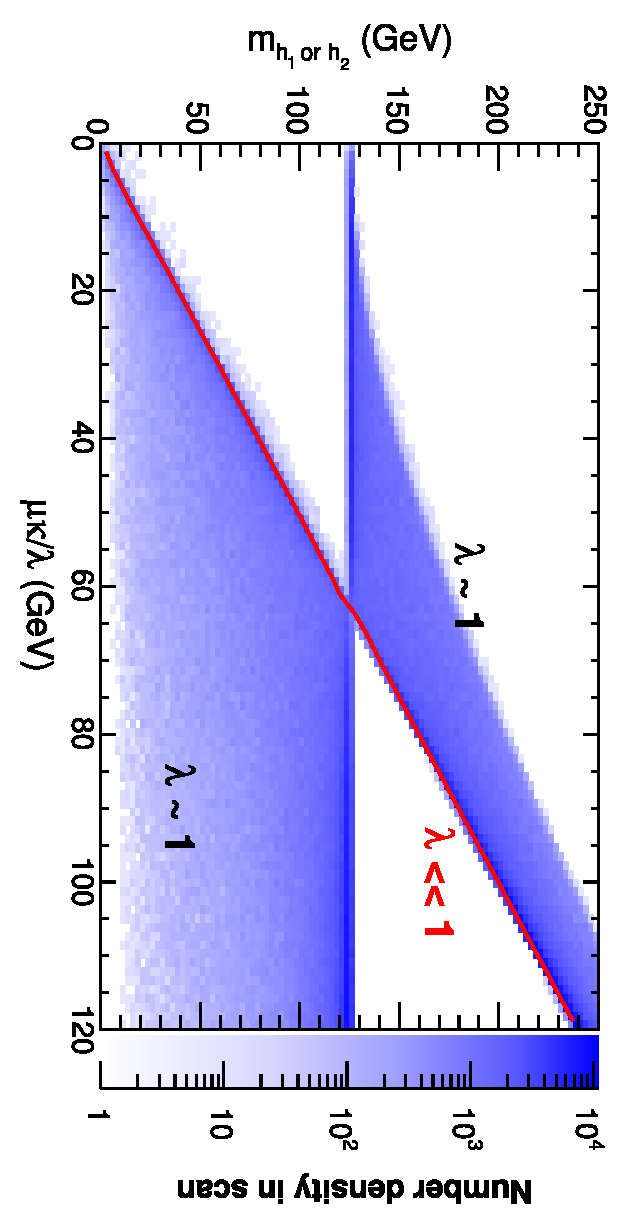
\includegraphics[width=0.48\linewidth]{plots/newbranching/smass12_vs_mkovel.eps}
%%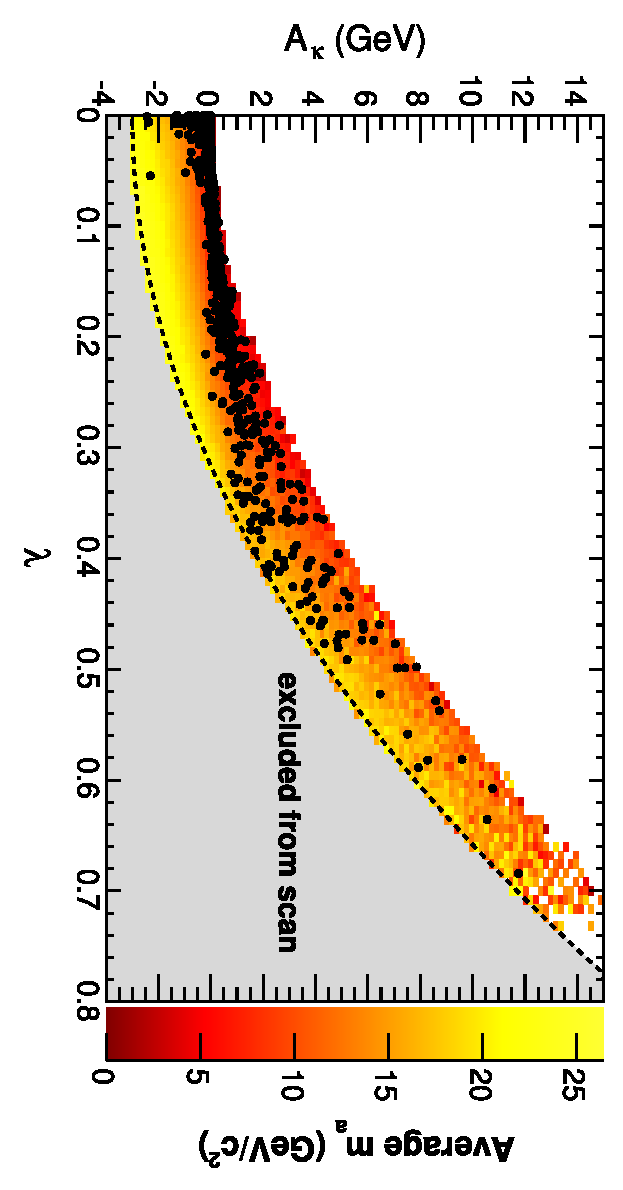
\includegraphics[height=0.48\linewidth, angle=90]{plots/newbranching/ma_vs_akappa_vs_lambda.eps}
\caption{(a): Lightest ($h_1$) and second-lightest ($h_2$) CP-even
  Higgs masses as a function of $\mu\kappa/\lambda$ and $\lambda$.
  The density of generated points surviving constraints is shown in
  the blue color scale, and the red line presents the single-valued
  $\lambda \ll 1$ limit.  (b): mass of the CP-odd Higgs ($m_a$) as a
  function of $A_\kappa$ and $\lambda$.  The color scale is the
  average mass in each bin, and filled circles are models with $m_a <
  2m_\tau$.  Low $m_a$ region follows the parabolic curve, $(\mbox{30~GeV})\lambda^2 - A_\kappa \ge 0$.
 \label{fig:hmass_mukoverl}}
\end{figure*}


\section{NMSSM Parameter Space}

%\subsection{The model and its parameters}
In our study we consider the simplest version of the NMSSM
\cite{Nilles:1982dy,Frere:1983ag,Ellis:1988er,%
Drees:1988fc,Ellwanger:1993hn,Ellwanger:1993xa,%
Elliott:1993bs,Pandita:1993tg,Ellwanger:1995ru,%
King:1995vk,Franke:1995tc,Ellwanger:1996gw},
in which the $\mu\widehat{H_1}\widehat{H_2}$ term of the 
MSSM superpotential is replaced by
\begin{equation}
\lambda  \widehat{S} \widehat{H}_1 \widehat{H}_2 + \frac{\kappa}{3}  \widehat{S}^3 \mbox{,}
\label{eq:superpot} 
\end{equation}
which makes the superpotential scale invariant.  In general, there are five
soft braking terms; in the "non-universal" case,
\begin{equation}
  m_{H_1}^2 H_1^2 + m_{H_2}^2 H_2^2  + m_{S}^2 S^2 
+ \lambda A_\lambda H_1 H_2 S +  \frac{\kappa}{3} A_\kappa S^3.
\label{eq:soft} 
\end{equation}
In the above equations, capital letters with tildes denote superfields
while symbols without tildes denote the scalar component of the respective
superfield.

Soft breaking parameters in Eq.(\ref{eq:soft}), $m_{H_1}^2$ , $m_{H_2}^2$  and $m_{S}^2$, 
can be expressed in terms of $M_Z$, the ratio  of the doublet Higgs vacuum expectation 
values (VEVs) $\tan\beta$, and $\mu = \lambda s$
(where $s=\langle S \rangle$, the VEV of the singlet Higgs field)
through the three minimization equations of the Higgs potential.
Assuming that the Higgs sector is CP conserving,
the NMSSM Higgs sector at the Electro-Weak (EW) scale is uniquely defined
by 14 parameters:
$\tan\beta$,
the trilinear couplings in the superpotential $\lambda$ and $\kappa$, the
corresponding soft SUSY breaking parameters $A_\lambda$ and $A_\kappa$,
the effective $\mu$ parameter $\mu = \lambda s$,
the gaugino mass parameters $M_1$, $M_2$ and $M_3$,
the squark and slepton trilinear couplings
$A_{t}$,  $A_{b}$ and  $A_\tau$,
and the squark and slepton mass parameters $M_{f_L}$ and $M_{f_R}$.
For simplicity, we assume here the
universality within 3 generations for the last two parameters, leaving
only 6 parameters for sfermion masses.

In particular, the above parameters define $\CM_{S}$ and $\CM_{P}$, the CP-even and CP-odd Higgs mass matrices, 
respectively~\cite{nmssmtools1}:
\begin{eqnarray}
\CM_{S11}^2 & = & g^2 v^2 \sin\beta^2 + \mu\cot\beta(A_\lambda + \kappa s ) 				\nonumber\\
\CM_{S22}^2 & = & g^2 v^2 \cos\beta^2 + \mu\tan\beta(A_\lambda + \kappa s )				\nonumber\\
\CM_{S33}^2 & = & \lambda A_\lambda \frac{v^2\sin 2\beta}{2s} + \kappa s(A_\kappa + 4\kappa s )   	\nonumber\\
\CM_{S12}^2 & = & (\lambda^2 - g^2/2) v^2\sin 2\beta -\lambda s (A_\lambda + \kappa s) 			\nonumber\\
\CM_{S13}^2 & = & \lambda v (2\lambda  s \sin\beta - \cos\beta (A_\lambda + 2\kappa s))			\nonumber\\ 
\CM_{S23}^2 & = & \lambda v (2\lambda  s \cos\beta - \sin\beta (A_\lambda + 2\kappa s))			
\label{eq:ms}
\end{eqnarray}
\begin{eqnarray}
\CM_{P11}^2 & = & {2\lambda s\over{\sin 2\beta}} (A_\lambda + \kappa s ) 				\nonumber\\
\CM_{P22}^2 & = & 2\lambda\kappa v^2 \sin 2\beta + \lambda A_\lambda {{v^2\sin 2\beta}\over{2s}} -3\kappa A_\kappa s \nonumber\\
\CM_{P12}^2 & = & \lambda v (A_\lambda - 2\kappa s )  
\label{eq:mp}
\end{eqnarray}

\subsection{Parameter Scan of the NMSSM Low-$m_a$ Region}

To find the parameter space for our region of interest, $m_a < 2m_\tau$, 
we scan the NMSSM parameter space using the NMSSMTools
package~\cite{nmssmtools1,nmssmtools2,nmssmtools3}, applying all known
phenomenological and experimental constraints except the following:
the cosmological dark matter relic density measured by WMAP~\cite{wmap}, 
direct $p\bar{p} \to h_1 \to aa \to 4\mu$ and $2\mu$, $2\tau$ searches by the
Tevatron~\cite{Abazov:2009yi}, 
direct $e^+e^- \to Zh_1$, $h_1 \to aa$ searches by
LEP~\cite{lep1exclusion,lep2exclusion}, and direct 
$\Upsilon \to \gamma a$ searches by CLEO~\cite{:2008hs}
and BaBar~\cite{Aubert:2009cp}.  
These important constraints will be applied explicitly to our region 
of interest in a later section.

\begin{figure*}[tbh]
%%\includegraphics[height=4 cm]{plots/newbranching/pcomp12.eps}
%%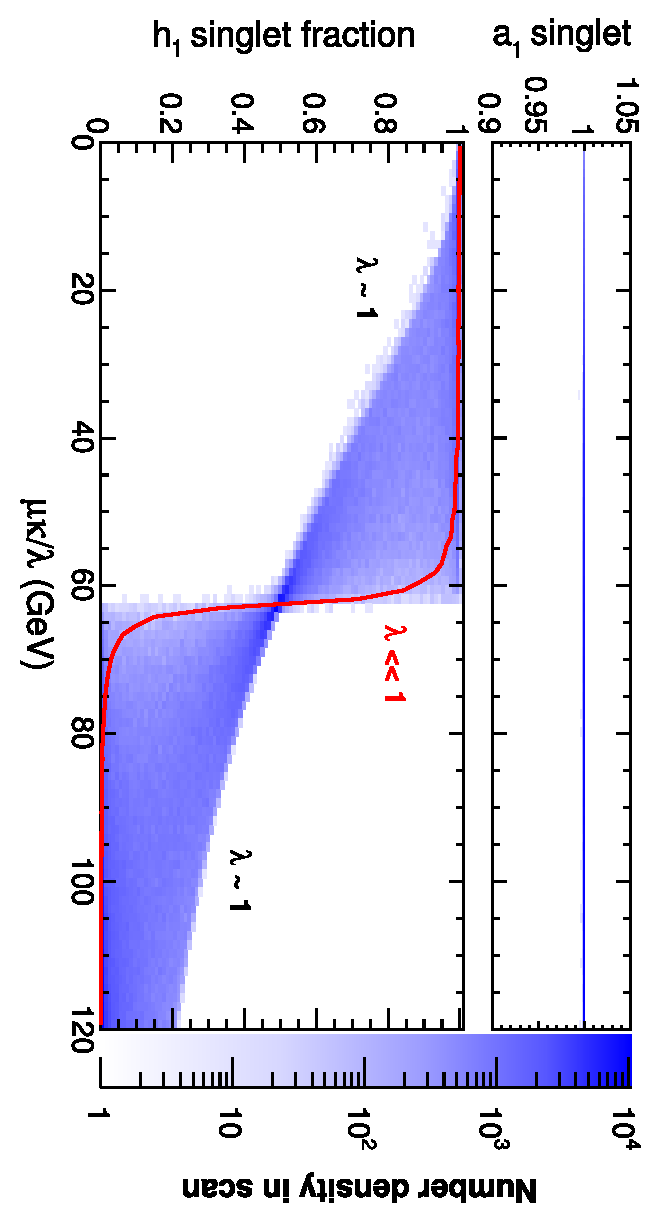
\includegraphics[height=4 cm]{plots/newbranching/scomp13_vs_mkoverl.eps}
\caption{(a): Non-singlet fraction of $a_1$ on a logarithmic scale: $a_1$
  is nearly a pure singlet {\bf for the entire parameter space}; (b): Singlet fraction of 
  $h_1$ as a function of $\mu\kappa/\lambda$. \label{fig:singlet}}
\end{figure*}

The scan was performed by sampling NMSSM model points uniformly in a six dimensional space determined by the 
following variables and ranges:
\begin{itemize}
\item 100~GeV $<$ $\mu$ $<$ 1000~GeV
\item 0 $<$ $\lambda$ $<$ 1
\item 1.5 $<$ $\tan\beta$ $<$ 50
\item $-$1~TeV $<$ $A_\lambda$ $<$ 5~TeV
\item 0 $<$ $\mu\kappa/\lambda$ $<$ 120~GeV
\item $-0.1$~GeV $<(\mbox{30~GeV})\lambda^2 -A_\kappa < 3$~GeV.
\end{itemize}
while the remaining parameters (entering the Higgs sector at loop-level) were
fixed at $M_1/M_2/M_3 = 150/300/1000$ GeV, $A_t = A_b = A_\tau = 2.5$ TeV, 
$M_{f_L}  = M_{f_L} =1$~TeV. The first four scan parameters are conventional,
broad ranges over the probable values of $\mu$, $\lambda$, $\tan\beta$, and
$A_\lambda$. We chose the fifth parameter of the scan equal to  $\mu\kappa/\lambda
= \kappa s$ since it is correlated with the mass of the CP-even higgs bosons
as one can see in Fig.~\ref{fig:hmass_mukoverl}(a).

Generally, $a_1$ is light if the parameters of the model are near Peccei-Quinn (PQ) symmetry limit ($\kappa\to 0$) 
or/and near the R-symmetry (RS) limit ($A_\kappa, A_\lambda\to 0$). In both limits, $a_1$ is a massless axion, 
as it directly follows from Eq.(\ref{eq:mp}). It can be decomposed in terms of the weak eigenstates $H_{uI}$, 
$H_{dI}$ and $S_I$ as (see e.g. \cite{Ellwanger:2009dp}):
\begin{equation}
a_1=c_{\theta_P} A + s_{\theta_P} S_I
\end{equation}
where $A=\cos\beta H_{uI} + \sin\beta H_{dI}$. In the case of PQ limit mixing parameters $c_{\theta P}$, 
$s_{\theta P}$ are:
\begin{equation}
c_{\theta_P} ={v \sin 2\beta\over{\sqrt{v^2\sin^2 2\beta+4 s^2}}},
s_{\theta_P} = -{2s\over{\sqrt{v^2\sin^2 2\beta+4 s^2}}}.
  \label{eq:pqmix}
\end{equation}
In the case of RS limit, the same parameters are:
\begin{equation}
c_{\theta_P} = {v \sin 2\beta\over{\sqrt{v^2\sin^2 2\beta+ s^2}}},
  s_{\theta_P} = {s\over{\sqrt{v^2\sin^2 2\beta+ s^2}}}.
  \label{eq:rsmix}
\end{equation}

{\bf Mass of $a_1$ is driven by $\CM_{P22}$ element in Eq.~(\ref{eq:mp})}. Using $m_{h1}\simeq 2\mu\kappa/\lambda$, 
that expression can be re-written as
\begin{eqnarray}
{{2}\over{3}} {{m_{a_1}^2}\over{m_{h_1}}} \simeq  \zeta \lambda^2 - A_\kappa, \; {\rm where} \; \zeta = {{v^2\sin 2\beta}\over{3\mu}} (2+{{A_\lambda}\over{m_{h_1}}}) \nonumber.
\end{eqnarray}
Therefore, $a_1$ is light if $(\zeta \lambda^2 - A_\kappa)$ is low, motivating the choice of the empirical parameter 
$(\mbox{30~GeV})\lambda^2-A_\kappa$ used in the scan. The range used in the scan for this parameter selects a region 
with a roughly uniform distribution of $m_{a_1}$ between 0 and 30~GeV and avoids most of the theoretically inaccessible 
region with $\zeta\lambda^2-A_\kappa<0$ where $m_a^2<0$. {\bf In this region $A_\kappa$ is limited to be small 
which is motivated by RS limit, pushing $a_1$ to be light. (is this right and relevant? - Alexei)}

{\bf In the region of interest (small $\lambda$ (???), $A_\lambda$ (???) and $A_\kappa$}), the mass of the lightest 
CP-even Higgs mass is determined by $\CM_{S33} \simeq 2\kappa s = 2\mu\kappa/\lambda$, see Eq.~\ref{eq:mp}. For 
$\mu\kappa/\lambda<60$ GeV, $h_1$ is light with the mass $m_{h1}\simeq 2\mu\kappa/\lambda$ as illustrated in 
Fig.~\ref{fig:hmass_mukoverl}(a), and has a significant singlet component, particularly for smaller values of 
$\lambda$ (and $A_\lambda$), which suppresses the doublet-singlet mixing. For $\mu \kappa/\lambda>60$ GeV,
$\CM_{S33}$ defines the mass of the $h_2$ Higgs boson, which aquires a large singlet component, while $h_1$ 
becomes the SM-like Higgs with $m_{h_1}\simeq120$ GeV. The upper bound on the scan parameter $\mu \kappa /\lambda<120$ GeV 
was therefore chosen to create two equal size but phenomeologically distinct sub-regions.

\begin{figure*}[thb]
%%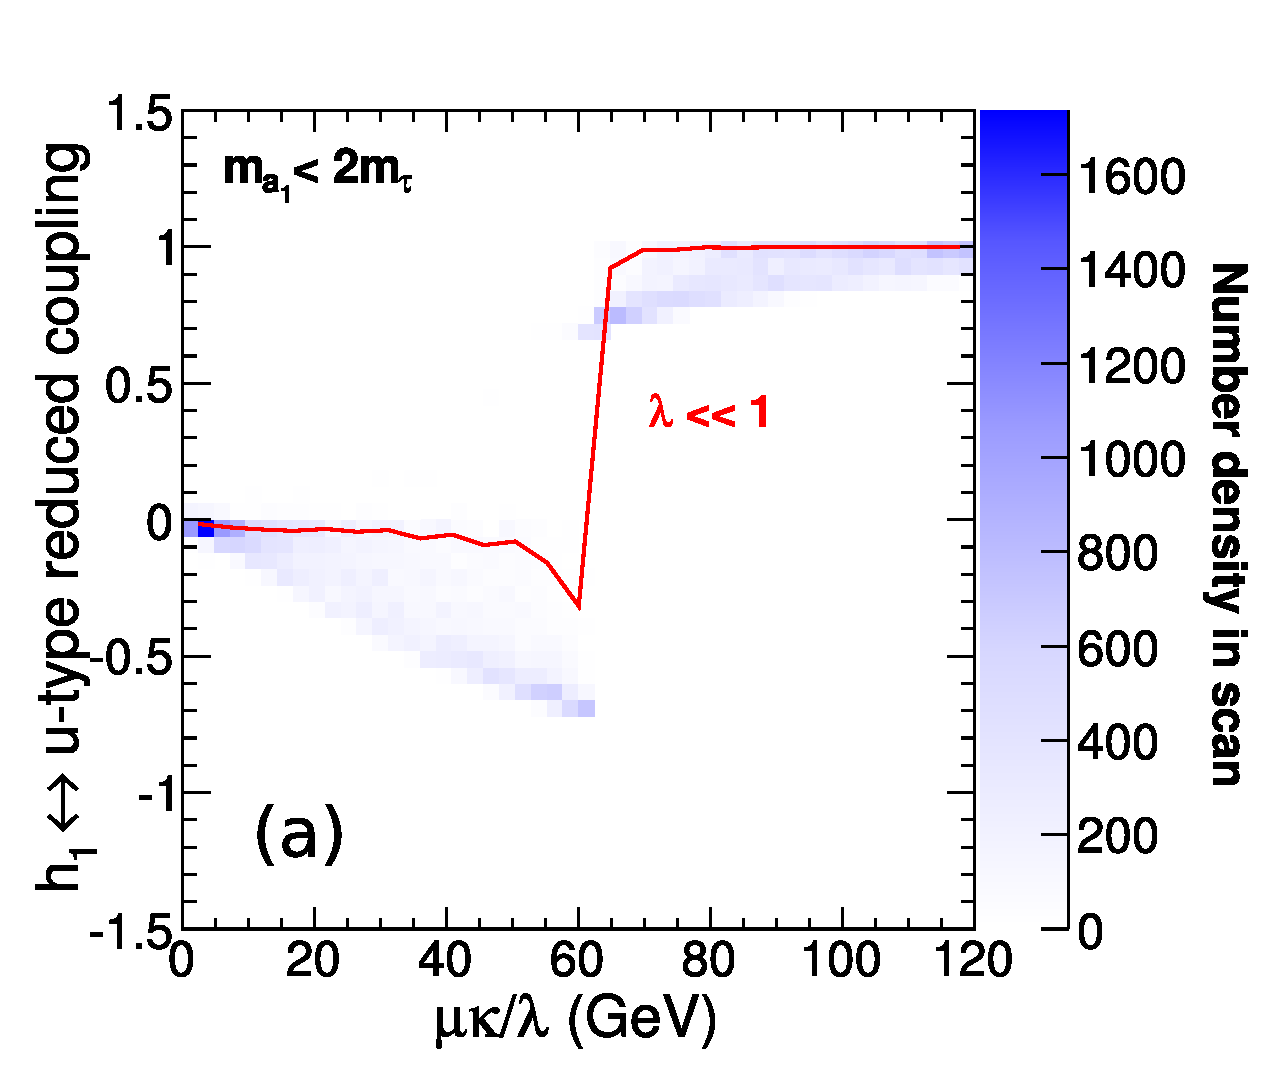
\includegraphics[width=0.32\linewidth]{plots/newbranching/cu1_vs_mkoverl.eps}
%%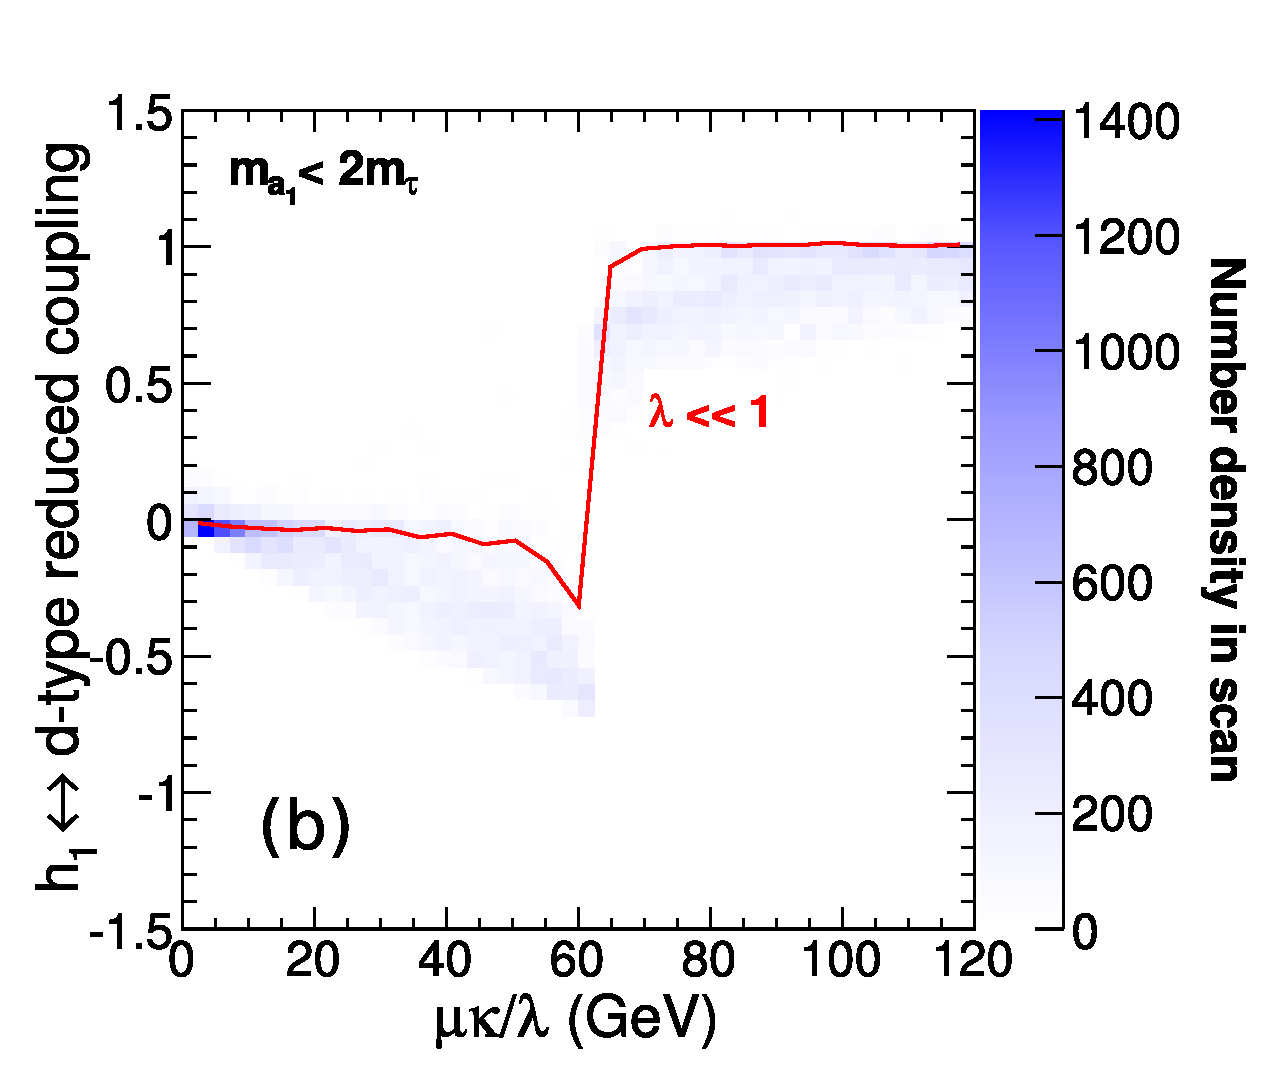
\includegraphics[width=0.32\linewidth]{plots/newbranching/cd1_vs_mkoverl.eps}
%%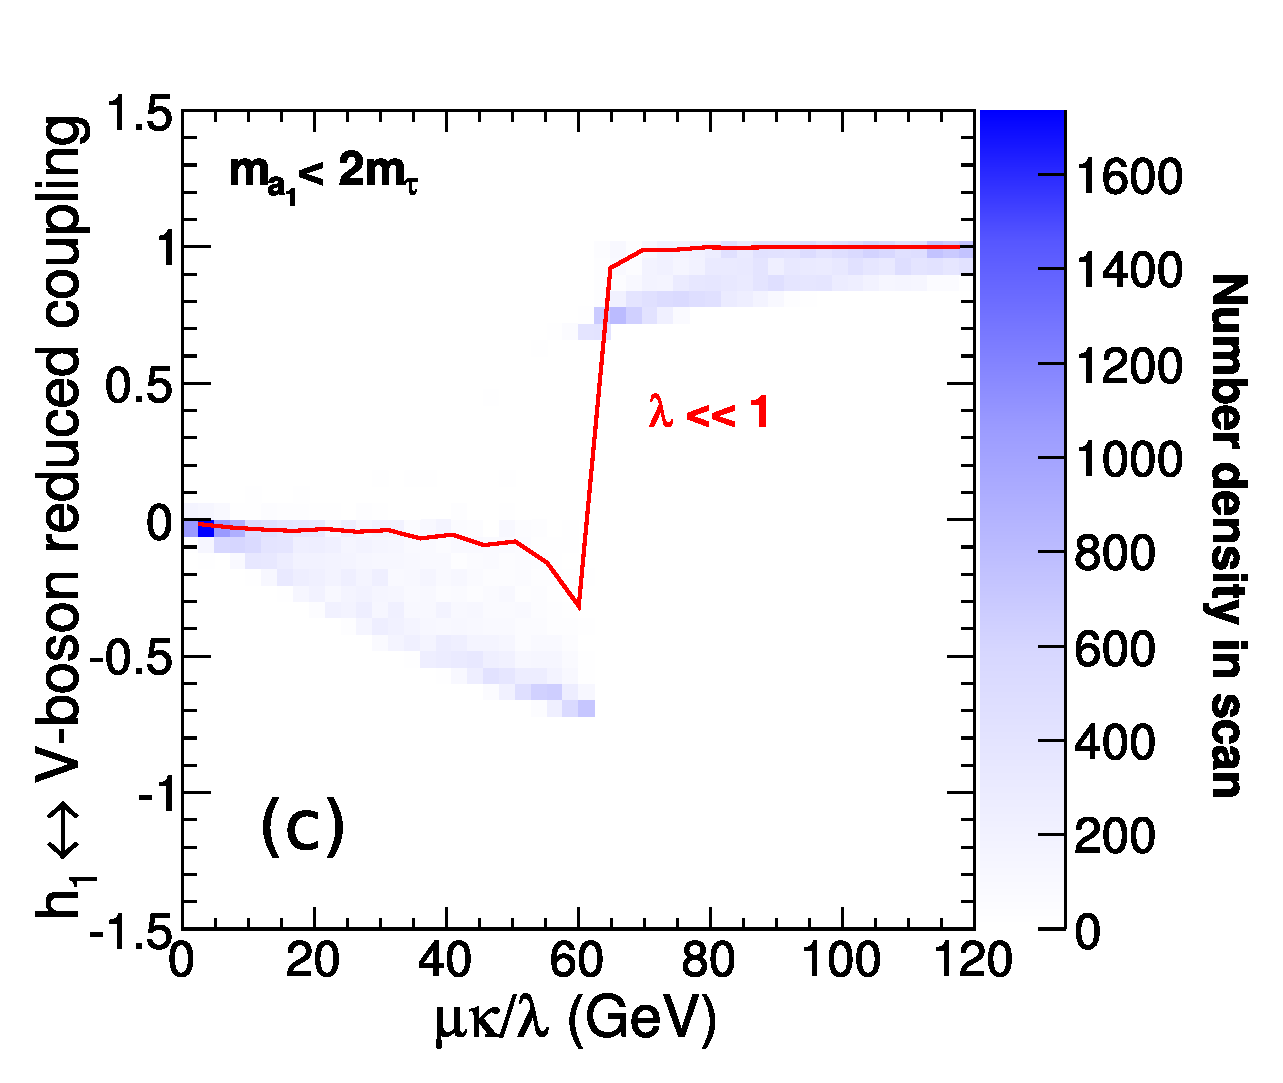
\includegraphics[width=0.32\linewidth]{plots/newbranching/cv1_vs_mkoverl.eps}
\caption{Reduced couplings of $h_1$ to up-type quarks (left), down-type
  quarks (middle), and vector bosons (right) as a function of $\mu\kappa/\lambda$, with
  the requirement that $m_a < 2m_\tau$.  The red line presents the
  single-valued $\lambda \ll 1$ limit. \label{fig:sm_mukoverl1}}
\end{figure*}

The couplings of $h_1$ and $a$ to each other and to Standard Model particles, are determined by their 
singlet and non-singlet componets. The CP-odd $a_1$ is nearly a pure singlet in both PQ and RS limits 
because $s=\mu/\lambda\gg v\sin 2\beta$ so that $s_{\theta_P} \simeq 1$, see Eq.(\ref{eq:pqmix}, \ref{eq:rsmix}). 
In fact, as shown in Fig.\ref{fig:singlet}(a), the non-singlet fraction $1-s_{\theta_P}^2  \lesssim 10^{-4}$ for 
the entire region of interest. {\bf Following bold text seems incomplete or out of context: Here we 
denote  $\SC_{13}$ as a mixing between the first ($H_{dR}$)
and  the third ($S_{R}$) CP-even Higgs boson weak eigensttaes.  
Increase of $\lambda$  enhances the  mixing of singlet and nonsinglet
Higgs boson eigenstates for both, CP-odd and CP-even Higgses. (let us plot  
$\log(1-s_{\theta_P})$ versus $log( v \sin 2\beta \lambda/\mu)$, where v =174 GeV) - SASHA}

The singlet fraction of $h_1$ (parameter $\SC_{13}^2$ in NMSSMTools) is primarily driven by 
$\mu\kappa/\lambda$ and $\lambda$, as illustrated in Fig.~\ref{fig:singlet}(b). 
In the small $\lambda$ limit, $h_1$ is nearly a pure singlet in the $\mu\kappa/\lambda \lesssim 60$~GeV
sub-region, while in the $\mu\kappa/\lambda \gtrsim 60$~GeV domain $h_1$ has negligible singlet component 
and is essentially the SM Higgs. Figure~\ref{fig:sm_mukoverl1} shows strong suppression of reduced couplings 
of $h_1$ to up- and down-type quarks as well as vector bosons in the $\mu\kappa/\lambda \lesssim 60$~GeV 
domain. This suppression leads to a severe reduction in the production rates of $h_1$ at colliders 
making this scenario challenging for experimental exploration.

Experimentally important branching fractions of $h_1$ are determined by relative strength of 
the $h_1$ couplings to SM particles and the new, specific to MSSM, $h_1 a_1 a_1$ coupling. 
Because $a_1$ has a very high singlet fraction, the singlet/doublet content of $h_1$ has 
a strong effect on the strength of the $h_1 h_1 a_1$ coupling. If this was the only effect,
$B(h_1 \to a_1 a_1)$ would have been close to 100\% in the lower half of the $\mu\kappa/\lambda$
domain and negligible in the upper half. However, this coupling is also proportional to 
$\lambda$ (see Eq.~\ref{eq:soft}), which creates a competing effect as larger values of 
$\lambda$ smear the nearly perfect separation of singlet- and doublet-type $h_1$ in the lower
and upper halfs of the $\mu\kappa/\lambda$ domain. The end result is illustrated in 
Fig.~\ref{fig:brhaa} showing average $B(h_1 \to a_1 a_1)$ for NMSSM models with $m_a< 2m_\tau$ 
as a function of $\mu\kappa/\lambda$ and $\lambda$. It is evident that the suppression of $h_1$ 
SM couplings for $\mu\kappa/\lambda < 60$ GeV makes $B(h_1 \to a_1 a_1)$ substantial as long as 
$\lambda$ is not too small. For the upper part of the $\mu\kappa/\lambda$ domain, $B(h_1 \to a_1 a_1)$ 
is small except only for large values of $\lambda$ where the $h_1$ singlet fraction is enhanced.

\begin{figure}[htb]
%%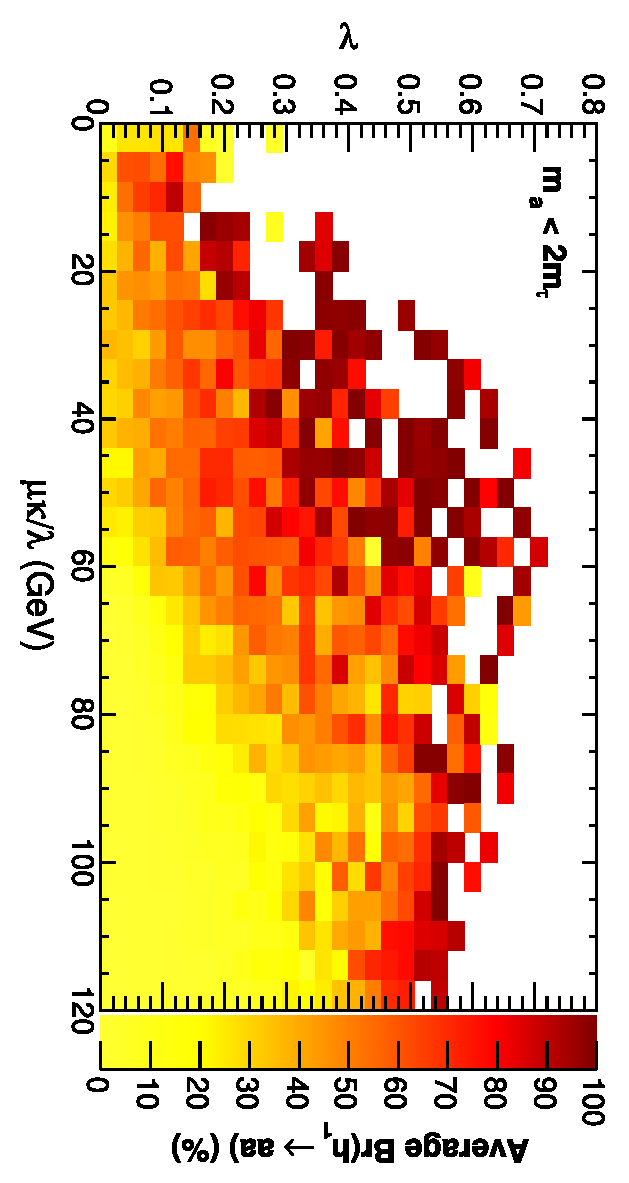
\includegraphics[height=0.95\linewidth, angle=90]{plots/newbranching/brhaa_vs_lambda_vs_mkoverl.eps}
\caption{Branching fraction of $h_1 \to a_1a_1$ in 
  the $\lambda$, $\mu\kappa/\lambda$ plane, with the requirement that $m_a <
  2m_\tau$. \label{fig:brhaa}}
\end{figure}

As the lightest Higgs boson, $a_1$ can only decay to SM particles. Coupling of nearly-singlet 
$a_1$ to all SM particles is strongly suppressed. This suppression is not universal in that 
the ratio of couplings of to up- and down-type quarks is about $1-3 \times 10^{-3}$ for the 
region of parameter space applicable to this study. As a result, $a_1$ branching fractions 
follow the standard mass hierarchy throughout our region of interest, except for a strong 
suppression of decays to the up-type quarks. {\bf (I think we need to say if the lifetime 
is affected or not, this seems as an obvious question. Do we have partial widths for $a_1$? We 
just need any one channel).} Figure~\ref{fig:bramm} shows the the branching fraction for 
$a \to \mu\mu$ as obtained using NMSSMTools package. For $m_a < 2m_\tau$ the $a \to \mu\mu$ 
channel becomes significant, making an analysis in the four muon mode viable for experimental 
searches. 

\begin{figure}[htb]
%%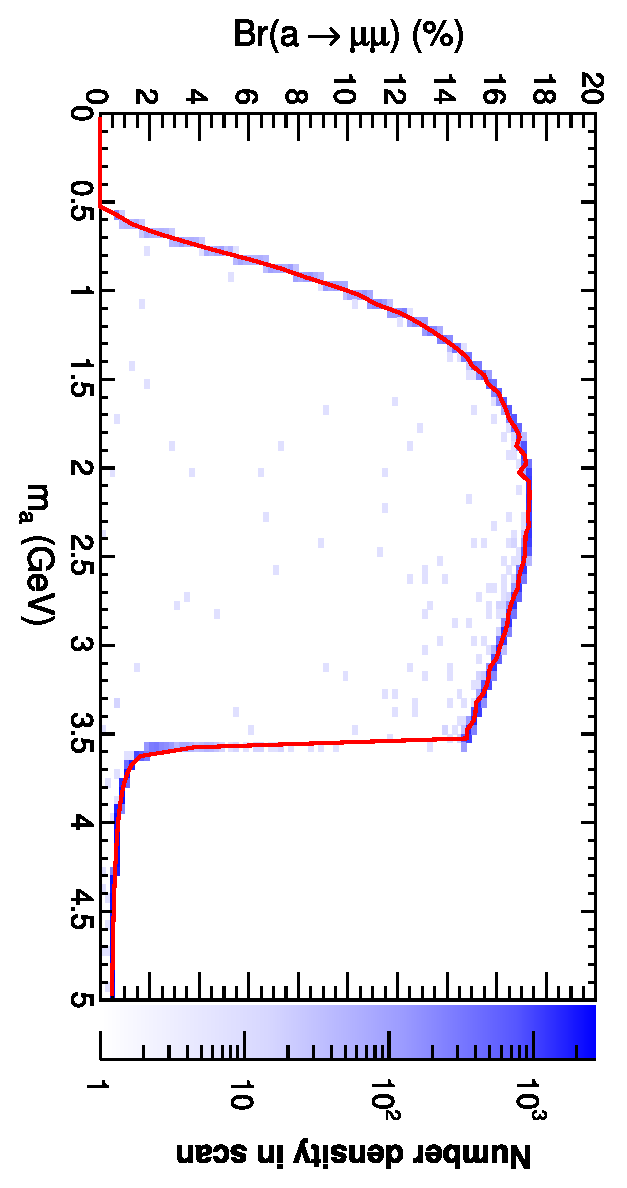
\includegraphics[height=0.95\linewidth, angle=90]{plots/newbranching/bra_vs_ma.eps}
\caption{ Branching fraction of $a_1 \to \mu \mu$ for generated
  models as a function of $m_a$.  The red line is the average as a
  function of $m_a$, demonstrating that the branching fraction is
  nearly a strict function of mass.  The threshold at 3.55~GeV is
  $2m_\tau$.  When $m_a < 3m_\pi$ (the grey box), the branching
  fraction to $\mu\mu$ becomes nearly 100\%. \label{fig:bramm}}
\end{figure}

\begin{figure*}[t]
%%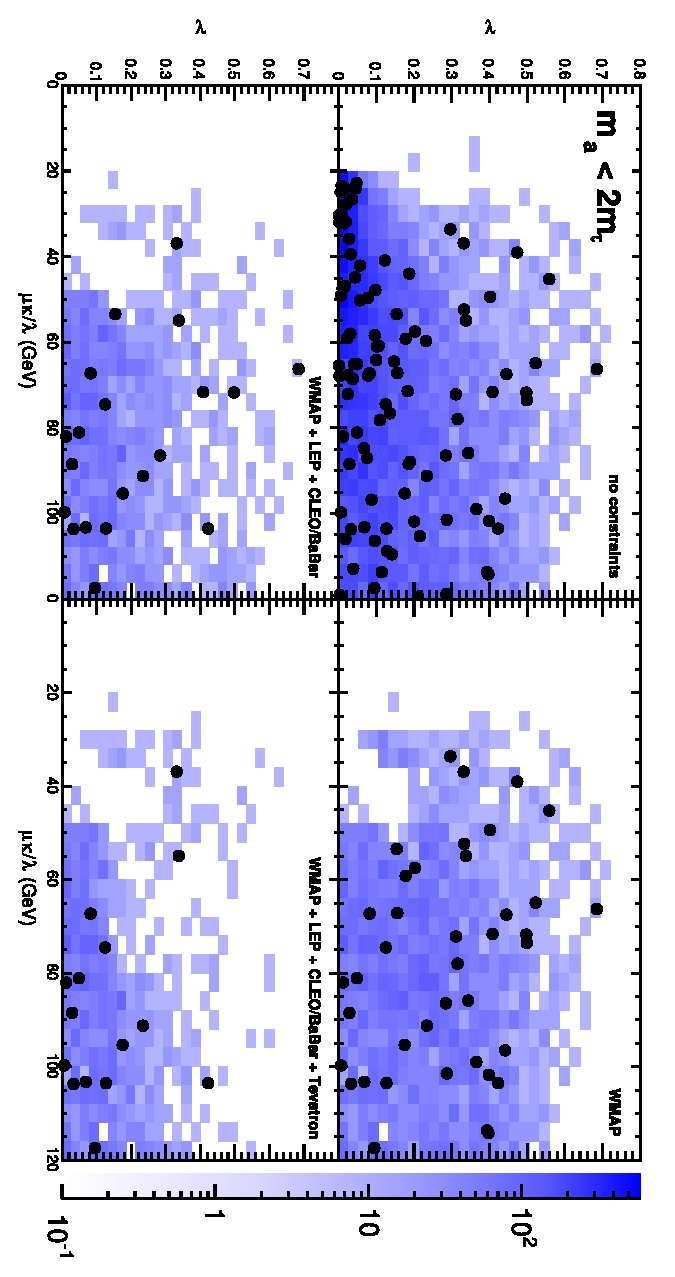
\includegraphics[height=0.8\linewidth, angle=90]{plots/newbranching/fourconstraints_params.eps}
\caption{Sampled points with $m_a < 2m_\tau$ and experimental constraints successively applied 
in $\lambda$ vs.\ $\mu\kappa/\lambda$ space. Note that the low energy $e^+e^-$ data (CLEO and
BaBar) have essentially no impact on the allowed parameter space. Color scale is number density 
and filled points are 100 models (before application of experimental 
constraints). \label{fig:exclusion_params}}
\end{figure*}

It is important to note that the NMSSMTools calculation of $B(a\to \mu \mu)$ shown in Fig.~\ref{fig:bramm} 
does not include hadronization effects important in the region $m_a<1$ GeV/c$^2$, 
and therefore requires certain corrections. First, for $m_a<3m_\pi$, $B(a \to \mu\mu)$ is 
expected to be very high because $q\bar{q}$ and $gg$ decays are prohibited by hadronization and 
spin effects {\bf need a reference?} and $\gamma \gamma$ is small {\bf (the preprint with BR's 
says that in LH $\eta$ does not couple to vector bosons, which makes $\gamma \gamma$ smaller, 
which may not be the case for us, it can explain the difference in BR below)}. As for the 
NMSSMTools prediction for $m_a>0.5$ GeV/c$^2$, we compared it with another 
calculation~\cite{LHiggsADecays} performed in the context of the Little Higgs model. 
The two calculations cannot be compared directly because the $c \bar{c}$ decay becomes 
dominant for $m_\eta>$2.5 GeV/c$^2$ in the Little Higgs case, while it is strongly suppressed 
in NMSSM. If corrected for this difference, calculation in~\cite{LHiggsADecays} seems to
predict $B(a_1 \to \mu \mu)$ of the order of 27\% instead of slightly under 20\% by NMSSMTools
and have a similar shape. {\bf( We should explain what was wrong in the recent paper by DZero
in using an incorrect $B(a \to \mu \mu)$. I am not sure here, Jim, could you draft the text?)}. 
For our numeric estimations, we choose to follow the NMSSMTools calculations shown in 
Fig.~\ref{fig:bramm}, but all results can be easily corrected if a different calculation
becomes available.

\subsubsection{Cosmological Constraints}

Lighest NMSSM neutralino becomes the candidate for the Cold Dark Matter (CDM). WMAP measurement of the CDM relic density 
therefore serves as an important constraint on the allowed NMSSM parameter space. 
In our scan, we used the MicrOmegas package~\cite{micrOmegas} linked to the NMSSMTools to calculate $\Omega_{NMSSM}$ 
to determine if a particular model is consistent with the experimental data. We considered a model to be consistent 
with the CDM measurement if $\Omega_{NMSSM} \le 0.1099 + 2\times0.0062$, which corresponds to the 95\% upper limit 
obtained using the latest WMAP 5-year dataset {\bf [ref]}. 

To illustrate the effect of WMAP constraints, Fig~\ref{fig:exclusion_params}(a) shows the density of generated
NMSSM models in the $\lambda$ versus $\mu\kappa/\lambda$ space under the constraint $m_{a_1}<2m_\tau$. Models 
that were determined to be consistent with the WMAP data are shown in Fig.~\ref{fig:exclusion_params}(b). The 
comparison shows that the WMAP bound excludes the region of small $\mu\kappa/\lambda$ and $\lambda$. In that region, 
the lightest neutralino is light and weakly interacts with SM particles. That suppresses neutralino annihilation 
rate enhancing the neutralino relic density to unacceptably large values. Figures~\ref{fig:exclusion_mass}(a) and (b)
make the same comparison but in the $m_{a_1}$ versus $m_{h_1}$ plane.

\begin{figure*}[t]
%%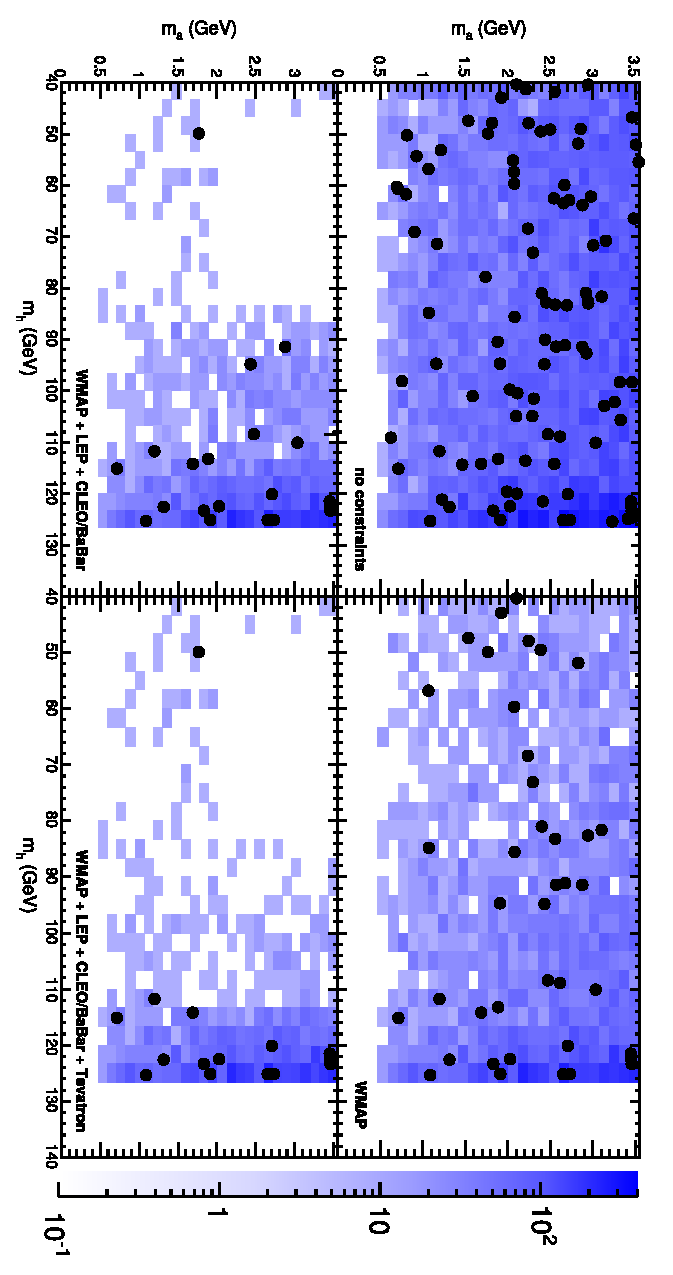
\includegraphics[height=0.8\linewidth, angle=90]{plots/newbranching/fourconstraints_masses.eps}
\caption{Sampled points with $m_a < 2m_\tau$ and experimental constraints successively applied 
similar to Fig.~\ref{fig:exclusion_params} but in $m_a$ vs.\ $m_h$ space.  Note that the low 
energy $e^+e^-$ data (CLEO and BaBar) have essentially no impact on the allowed parameter space. 
Color scale is number density and filled points are 100 models (before application of experimental 
constraints). \label{fig:exclusion_mass}}
\end{figure*}

\subsubsection{Constraints from Direct Searches at Colliders}

Several searches for NMSSM have been performed at collider experiments. The strongest impact on the allowed NMSSM models
comes from the LEP data. Although the large singlet component of $h_1$ at low $\mu\kappa/\lambda$ (and correspondingly 
low $m_{h_1}$) strongly suppresses $h_1$ production at LEP, relevant scenarios surviving WMAP constraints typically 
have sufficiently large $\lambda$, which enhances the doublet component of $h_1$ to the level sufficient to exclude 
$h_1 \to aa$ within the kinematic limits of $e^+e^- \to Z h_1$, $45 < m_{h_1} < 86$~GeV, and the detector efficiency 
for light CP-odd Higgs bosons, $m_a > 2$~GeV [ref]. In addition to LEP data, there have been several recent attempts 
aimed at direct searches at colliders. Searches at lower energy $e^+e^-$ colliders~\cite{cleo-low-ma,babar-low-ma} 
have been focusing on searching for the CP-odd Higgs via $\Upsilon \to \gamma a_1$ followed by the decay of $a_1$ 
to muons. Neither of these searches constrain the NMSSM models with low $m_a$ because the high singlet component of 
$a_1$ (see Fig.~\ref{fig:singlet}(a)) leads to negligible $bba_1$ coupling thus precluding production of $a_1$
at the low energy $e^+e^-$ colliders. Because CLEO and BaBar results have no effect on the allowed parameter space,
Figs.~\ref{fig:exclusion_params}(c) and~\ref{fig:exclusion_mass}(c) show combined LEP+CLEO+BaBar constraints, but 
the reader is reminded that only LEP constraints are important.

Results of a search~\cite{d0-low-ma} for NMSSM with a low mass $a_1$ at the Tevatron was recently published by the $D\O$ 
experiment in the channel $h_1 \to a_1 a_1 \to \mu \mu \mu \mu$. With no excess of data over the SM expectations, the 
paper quotes 95\% C.L. upper limits for the cross-section of this process. To interpret the $D\O$ result in terms of constraints 
on allowed NMSSM models in our scan, we calculate the NLO production cross-section for $p \bar{p} \to h_1$ in NMSSM using 
the SM NLO calculations for $gg \to H_{SM}$~\cite{Spira:1995rr} and $b\bar{b} \to H_{SM}$ with QCD-improved (running) Yukawa 
couplings~\cite{Balazs:1998sb} corrected for differences in coupling between SM and NMSSM using the NMSSMTools:
\begin{eqnarray}
\sigma(gg\to h_1)=\sigma(gg\to H_{SM})\frac{\Gamma(h_1\to gg)}{\Gamma(H_{SM}\to gg)} \\ \label{eq:ggcross_section}
\nonumber =\sigma(gg\to H_{SM})\frac{Br(h_1\to gg)\Gamma^{tot}(h_1)}{\Gamma(H_{SM}\to gg)} \\
\sigma(b\bar{b}\to h_1)=\sigma(b\bar{b}\to H_{SM})
\left(\frac{Y_{bbh_1}}{Y_{bbH_{SM}}}\right)^2 \label{eq:bbcross_section} 
\end{eqnarray}
where $\sigma(gg\to H_{SM})$ and $\Gamma(H_{SM}\to gg)$ is calculated using
HIGLU, while $Br(h_1\to gg)$, $\Gamma^{tot}(h_1)$, and the ratio of Yukawa couplings 
$Y_{bbh_1}/Y_{bbH_{SM}}$ are obtained using NMSSMTools. It turns out that for $\mu\kappa/\lambda<60$ 
(non-SM $h_1$ lighter than 120 GeV), the cross-section is strongly suppressed even compared to SM 
for low $m_a$ because $h_1$ has a large singlet fraction and weakly couples to SM partciles 
(see Fig.~\ref{fig:sm_mukoverl1}). For larger $\mu\kappa/\lambda$ the lighest 
CP-even higgs $h_1$ becomes the SM-like Higgs and has small $h_1 \to aa$ branching. 

The paper~\cite{d0-low-ma} quotes the 95\% C.L. limits on $\sigma(p\bar{p} \to h_1) \times B_{h_1 \to aa \to \mu\mu\mu\mu}$ 
for several choices of $m_{a_1}$ calculated for $m_{h_1}=100$ GeV/c$^2$. To determine if a particular model in our scan
is excluded by data, we linearly interpolate the published cross-section limits for values of $m_{a_1}$ 
between the points in~\cite{d0-low-ma}. To obtain the experimental cross-section limits as a function of $m_{h_1}$, we 
need to correct for the variations in experimental acceptance. We obtain those limits by taking the analysis acceptance 
to be linear versus $m_{h_1}$ ``increasing by $\sim$10\% when $m_{h_1}$ increases from 
80 to 150~GeV''~\cite{d0-low-ma} and matching it to the full analysis acceptance given at $m_{h_1}=100\;\gevcc$. We 
then calculate the production cross-section and branching ratios for the model points and compare it to the 
value we derived from~\cite{d0-low-ma}. Figures~\ref{fig:exclusion_params}(d) and~\ref{fig:exclusion_mass}(d) 
show the density of NMSSM models surviving WMAP, LEP and Tevatron constraints. Because of the suppression in
the production rate at lower $\mu\kappa/\lambda$ and small $B(h_1 \to a_1 a_1)$ at high $\mu\kappa/\lambda$, the 
Tevatron search has only a limited impact on the allowed NMSSM parameter space, mainly constraining models with high 
$\lambda$. A significant improvement in Tevatron reach for NMSSM would require a large increase in integrated luminosity 
likely leaving it up to the LHC to make a definitive discovery or exclusion of NMSSM models with low $m_a$.

\begin{figure*}[t]
%%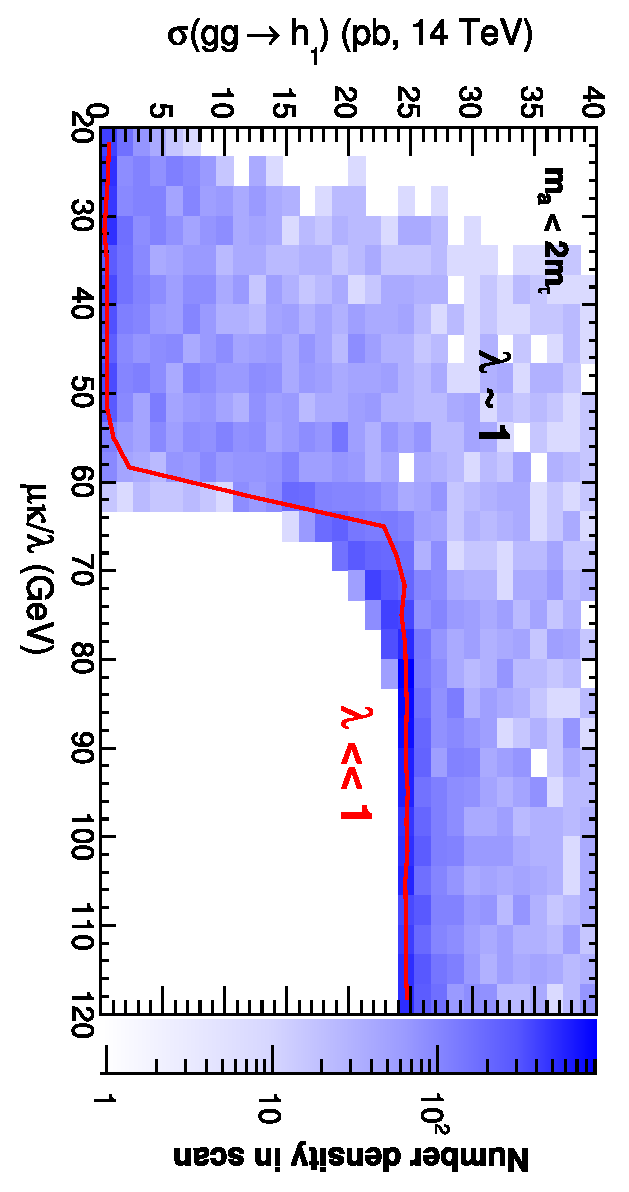
\includegraphics[width=0.48\linewidth]{plots/newbranching/crosssec_vs_mukoverl_gg.eps}
%%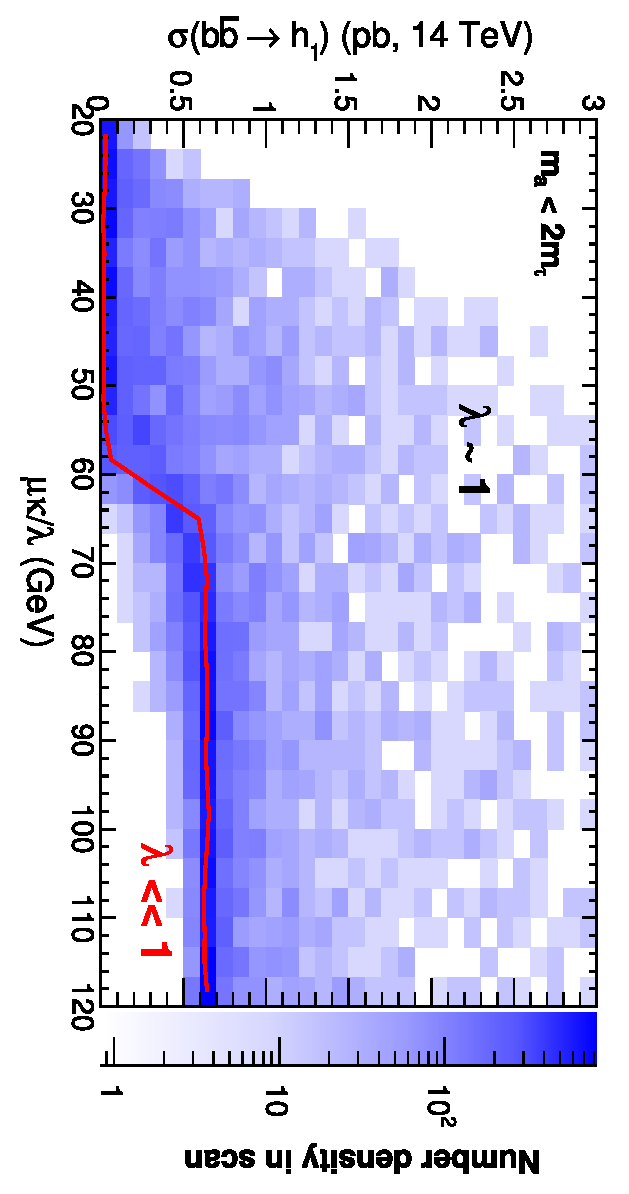
\includegraphics[width=0.48\linewidth]{plots/newbranching/crosssec_vs_mukoverl_bb.eps}
%%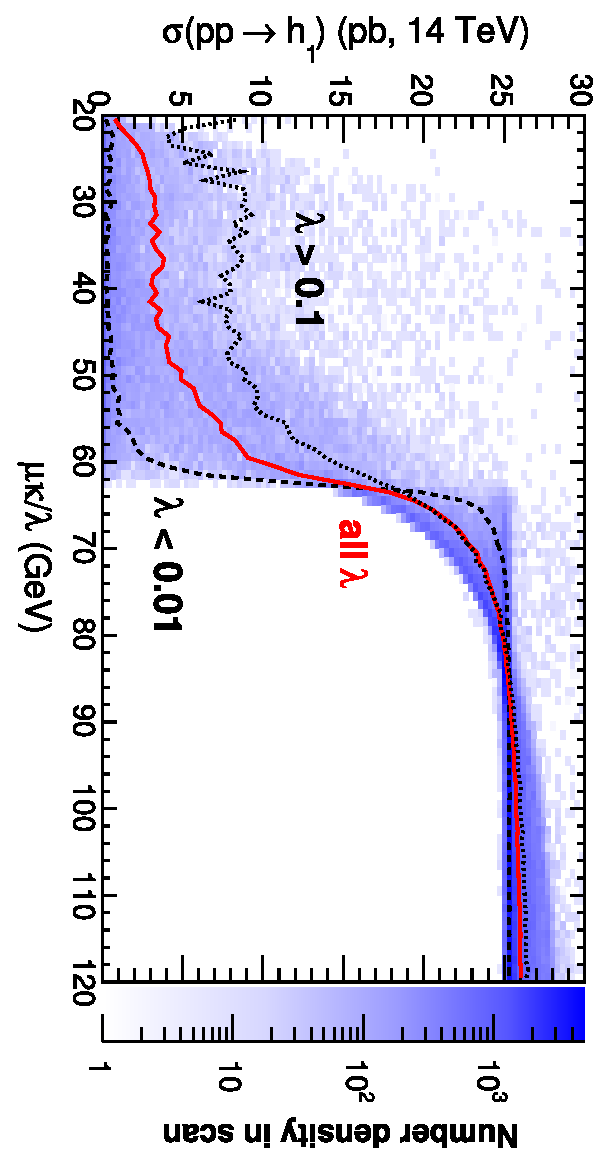
\includegraphics[height=0.7\linewidth, angle=90]{plots/newbranching/crosssec_vs_mukoverl.eps}
\caption{14~TeV production cross-section of $h_1$ as a function of
  $\mu\kappa/\lambda$ and $\lambda$, from $gg$ (left) and $b\bar{b}$
  (right), with the requirement that $m_a < 2m_\tau$.  The red line represents the single-valued $\lambda \ll 1$ limit.
  \label{fig:sm_mukoverl2}}
\end{figure*}

\subsection{Summary}
Existing experimental data provides important constraints on the NMSSM parameter space for models with low $m_{a_1}$. 
Particularly, WMAP data excludes many models with very low $\lambda$, particularly in the lower part of the $\mu\kappa/\lambda$
range. These scenarios are difficult for collider searches due to a large suprpession in cross-section production in
the low $\mu\kappa/\lambda$ domain and and small brnaching fraction $B(h_1 \to a_1 a_1$ for larger $\mu\kappa/\lambda$. 
Nevertheless, LEP data allows nearly complete exclusion of models with low $\mu \kappa / \lambda$ (light $m_{h_1}$) and 
$m_{a_1}>2$ GeV/c$^2$. Tevatron data further excludes a fraction of models with large $\lambda$. CLEO and BaBar data have
little if any effect on these NMSSM models as direct production for $a_1$ is extremely suppressed due to its high singlet
component. A large fraction of the parameter space still survives all these constraints leaving it up to the LHC to
either discover or exclude these models. Conclusive exclusion or discovery of new physics in this scenario would require 
a dedicated analysis performed at LHC. In the following, we propose the outline of such analysis and estimate its 
sensitivity.

\section{A Dedicated Search for the Low $m_{a_1}$ NMSSM at the LHC}

Because $a_1$ is dominated by the singlet component, it can only be produced at the LHC via decays of light Higgs 
$h_1 \to a_1 a_1$. The main characteristic of such signal at the LHC is two back-to-back (in $\phi$) di-muon pairs 
with pairs consisting of spatially close muons. The di-muon pairs, if reconstructed, should have invariant masses 
consistent with each other and also serves as a direct measurement of $m_a$. Additionally, the four muon invariant mass 
distribution should have a narrow spike corresponding to the $m_h$ mass. We use these striking features of signal 
events in designing the analysis suitable for early LHC running.

Experimentally, the four muon final state considered in this analysis is a very clean signature 
with relatively low backgrounds. Therefore, instead of using the Vector Boson Fusion (VBF)
chosen in earlier NMSSM searches targeting the $m_a>2 m_\tau$ region {\bf [ref]}, we focus on the largest 
Higgs production modes at the LHC, $gg \to h_1$ and $b\bar{b} \to h_1$.  We calculate the NLO 
cross-section for $pp \to h_1$ for NMSSM by rescaling the LHC SM NLO calculations~\cite{Spira:1995rr,Balazs:1998sb} 
to correct for differences in couplings between SM and NMSSM (Eqs.~\ref{eq:ggcross_section} and~\ref{eq:bbcross_section}). 
Similar to the Tevatron case, the cross-section is strongly suppressed compared to SM if $h_1$ 
has a large singlet fraction. Figure~\ref{fig:sm_mukoverl2} shows the production cross-section for 14~TeV $pp \to h_1+X$ 
as a function of $\mu\kappa/\lambda$.  While this large suppression makes this analysis challenging even at the LHC,
the constraints arising from the WMAP relic density measurement exclude models with very low values of $\lambda$, so
that the allowed models have small but not negligible production cross-section.

\subsection{Analysis Selections}
We use Pythia to generate signal event templates with $m_h$ in the range from 70 to 140 GeV/c$^2$
and $m_a$  in the range from 0.5 to 4 GeV/c$^2$. We chose the CMS detector as a benchmark for modeling
a realistic experimental environment and use parameters described in {\bf [ref CMS TDR}. The key 
parameters important for this analysis are muon momentum resolution, low threshold on muons to 
reach the muon system, acceptance and the average muon reconstruction efficiencies. Because of the
large number of reconstructed muons in the event, we take the trigger efficiency to be 100\%.

\begin{figure*}[htbp]
\begin{center}
%%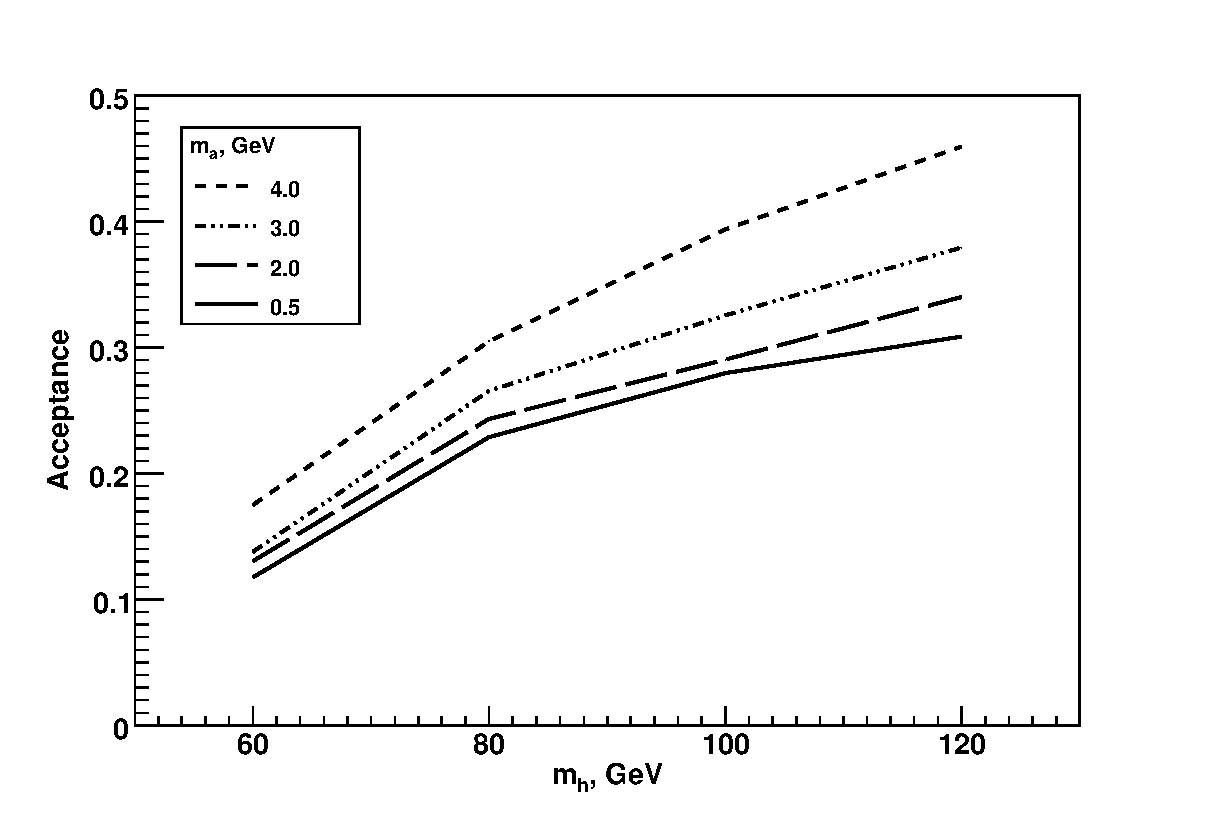
\includegraphics[width=0.48\linewidth]{plots/acceptance_vs_mh.eps}
%%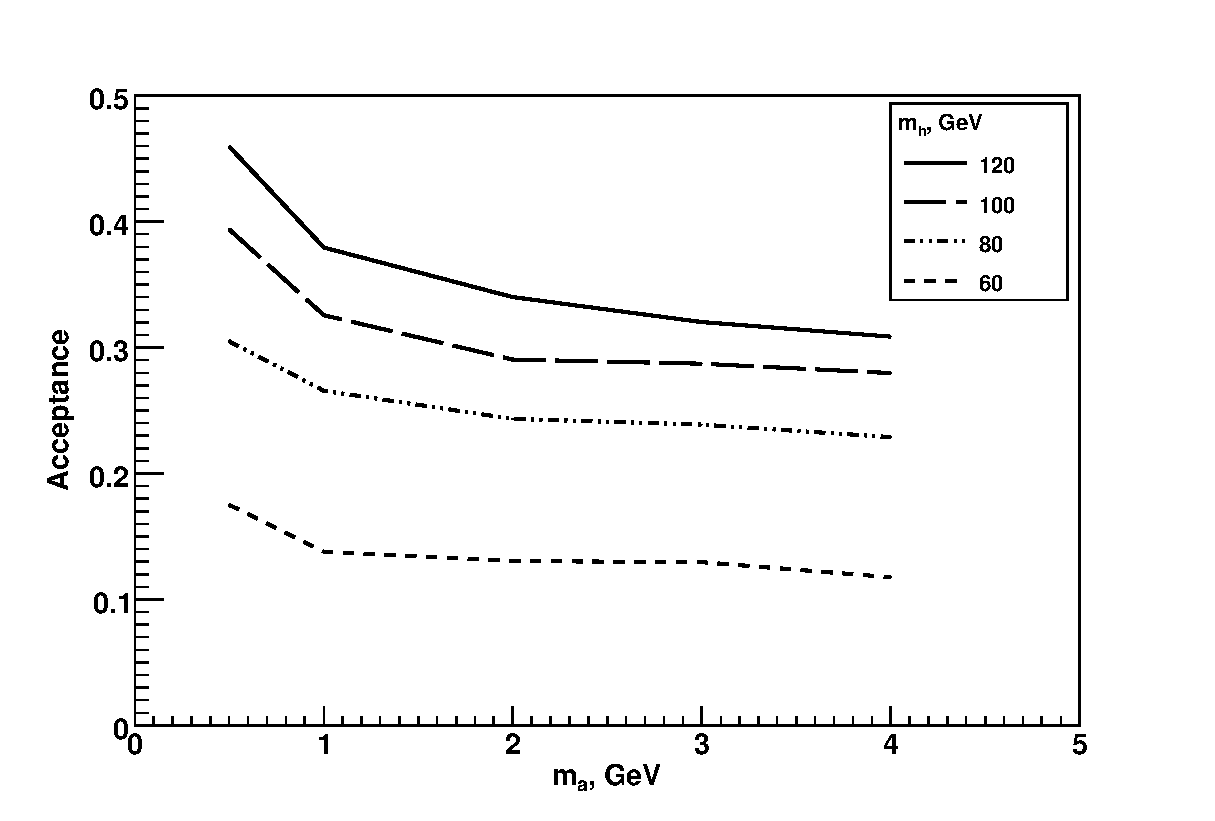
\includegraphics[width=0.48\linewidth]{plots/acceptance_vs_ma.eps}
\caption{Acceptance as a function of $m_a$ for fixed $m_h$. Acceptance as a function of $m_h$ for fixed $m_a$.}
\label{signal_acceptance}
\end{center}
\end{figure*}

The analysis starts by requiring at least four muon candidates with $p_T>5\;\gevc$ in the fiducial 
volume of the detector $|\eta|<2.4$, of which at least one has to have $p_T>20$ $\gevc$ to suppress 
major backgrounds and to satisfy trigger requirements. Each event must have at least two muon 
candidates of positive and negative charge each. For surviving events, we define quadruplets of 
candidates consisting of two positive and two negatively charged muon candidates. Next, we sort the 
four muon candidates in quadruplet into two di-muon pairs by minimizing the quantity 
$(\Delta R(\mu_i,\mu_j)^2 + \Delta R (\mu_k,\mu_l)^2)$, where $\Delta R^2 = \Delta \eta^2 + \Delta \phi^2$, 
under the constarint that each di-muon pair consists of two muon candidates of opposite charge. Muon
quadruplets, for which $\Delta R$ between muons in any of the two pair exceeds 0.5, are discarded as 
inconsistent with signal topology. Acceptance for the selections listed above is shown in 
Fig.~\ref{signal_acceptance} for several representative choices of values for $m_h$ and $m_a$. 

The requirement of four sufficiently energetic muons in the event drastically reduces contributions of 
potential backgrounds for this analysis. After acceptance selections, the dominant background is 
due to the QCD multijet production where muons originate from either heavy flavor quark decays or from 
$K/\pi$ decays in flight. We use Pythia to estimate the QCD multijet background and we estimate it
at this stage to be approximately 2.6 events/pb$^{-1}$ (approximately half due to true muons and the 
rest from events with both prompt muons and muons from decays in flight). We also considered electroweak 
backgrounds estimated using CompHEP {\bf [ref]} $pp \to 4l+X$ process to be 0.04 events/pb$^{-1}$ and direct J/psi 
production (Pythia), which was found to be completely negligible. Other SM backgrounds (top, W+jets) 
are negligible in the region of interest of this analysis.

The backgrounds are further reduced by applying kinematics requirements consistent
with the expected signal siganture. We calculate invariant mass of each of the di-muon pair, 
$m_{12}$ and $m_{34}$, as well as the invariant mass of all four muons denoted as $M$. Figure 
\ref{muon_pairs_masses_invariant_mass}a) shows the invariant mass of the muon pairs passing 
all selections in signal events for two choices of $m_h$ and $m_a$. Figure \ref{muon_pairs_masses_invariant_mass}b) 
shows the distribution of the invariant mass $M$ of the four muon system for two benchmark points. 
To focus on the region of interest, we require $M>60$ \gevcc, $m_{12}, m_{34} < 4$ $\gevcc$, which
reduces the QCD background to 0.4 events/pb$^{-1}$. 

\begin{figure*}[htb]
\begin{center}
%%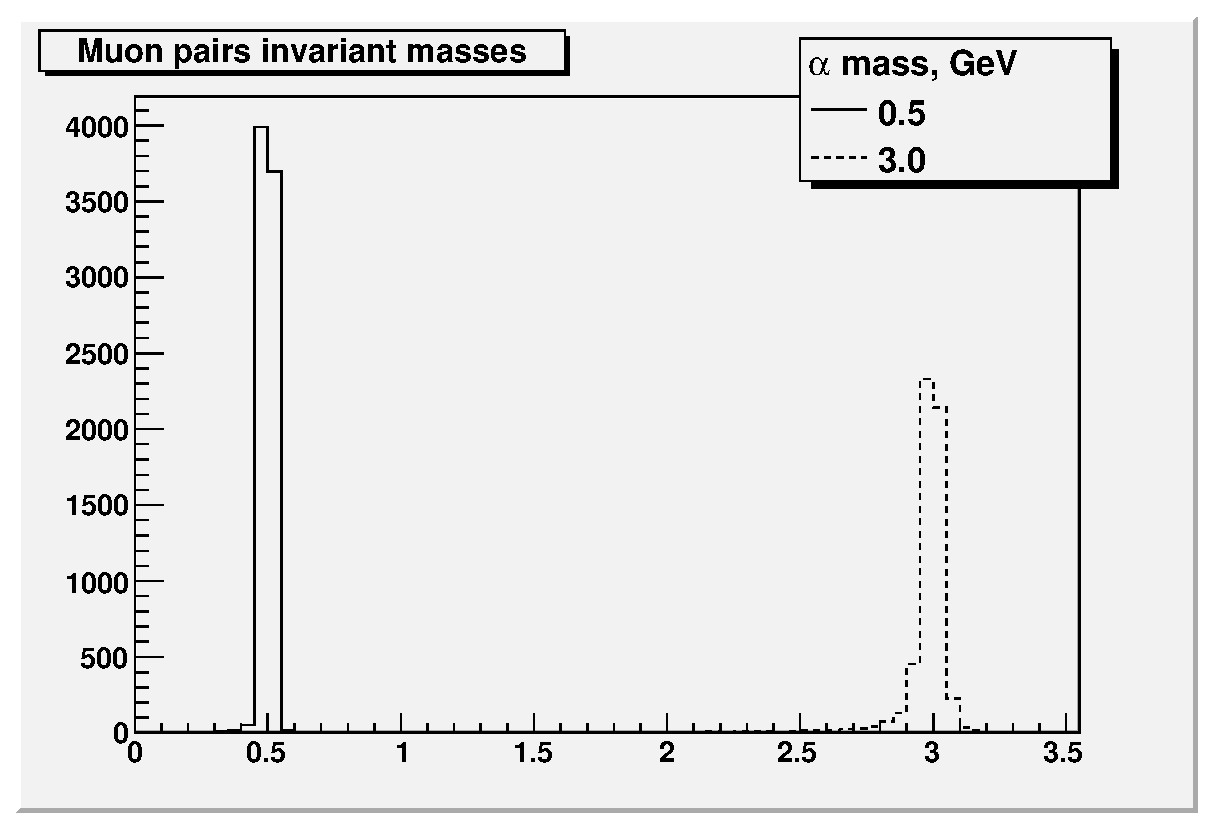
\includegraphics[width=0.48\linewidth]{plots/muon_pairs_masses.eps}
%%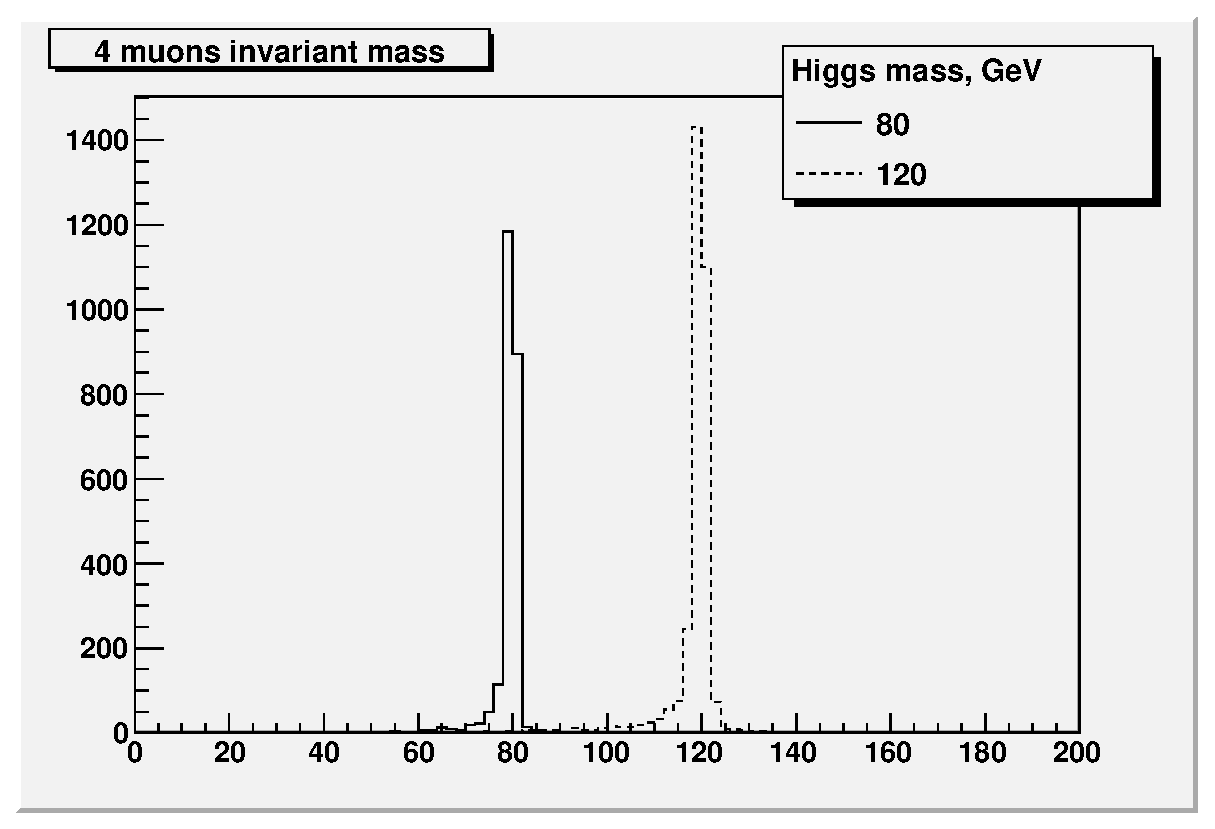
\includegraphics[width=0.48\linewidth]{plots/invariant_mass.eps}
\caption{Left: Reconstructed invariant mass of reconstructed muon pairs for $m_a=0.5$ and 
3 GeV/c$^2$ (in both cases $m_H$ = 100 GeV/c$^2$). Right: Reconstructed invariant of four muons for 
$m_H=80$ and $m_H=120$ GeV/c$^2$ (in both cases $m_a$ = 3.0 GeV).}
\label{muon_pairs_masses_invariant_mass}
\end{center}
\end{figure*}

To ensure the compatibility of the measured invariant masses of the two di-muon pairs, one could 
require $|m_{12}-m_{34}|<0.08+0.005*(m_{12}+m_{34})$. Such cut would enforce the requirement 
that the two pair masses are consistent with each other and takes into account widening of the 
absolute resolution in the reconstructed di-muon mass as a function of mass. If applied, the 
only background that still may be not completely negligible is the QCD multi-jet production, 
for which we conservatively estimate the upper bound to be 0.02 events/pb$^{-1}$. However, 
instead of applying this selection explicitly, a better approach would be to fit the data in 
the 3D space of measured values of $(m_{12},m_{34}, m_{1234})$ taking into account
kinematical properties of signal events. This approach allows maximizing signal
acceptance and therefore statistical power of the analysis. It is also convenient from 
experimental standpoint as the background events are distributed in a smooth fashion over the 
3D space allowing fitting the 3D distribution to estimate backgrounds directly from the data. 
Potential signal would appear as a concentration of events in one specific region in the 3D 
space (a 3D ``bump''). We use a binned likelihood defined as a function of parameters $m_a$, 
$m_h$ and effective signal cross section $\sigma \times B (h \to aa) B^2(a \to \mu \mu)$. 
Thus defined likelihood is used to fit pseudodata generated using either background or 
signal+background templates. We estimate sensitivity of the proposed analysis and present 
it in terms of the 95\% C.L. exclusion levels for signal cross-section using Bayesian 
technique.

Our estimations show that for an early data search ($L\simeq100$ pb$^{-1}$), the backgrounds are negligibe.
For analysis with higher luminosity, one can return back to the zero background situation by adding the 
isolation requirement to one or both of the di-muon pairs in the event. Isolation can be defined by 
either setting the upper bound on the sum of transverse momenta of all tracks in a cone around the 
reconstructed direction of the di-muon pair excluding momenta of the two muon tracks, or by rejecting pairs 
with additional tracks above a certain threshold. For our projections for an analysis with $L=1$ fb$^{-1}$, 
we required no charged tracks with momentum $p_T>1$ GeV in the cone of $\Delta R = \sqrt{(\Delta \eta)^2+\Delta \phi)^2}=0.3$ 
around the direction of at least one of the two muon pairs. This requirement is 96\% efficient for signal and 
reduces QCD multijet background, dominated by events with muons originating from heavy flavor 
jets, by a factor of 6-7. For high luminosity datasets, isolation can be further tightened to 
increase background suppression with only a moderate loss in signal efficiency.

\begin{table}[t]
\caption{Expected rate of background events per 100 $\ipb$ of luminosity after the selection cuts.\label{bckgr_cuts_number_reco_level}}
\begin{center}
%% \begin{tabular}{|c|c|c|}
%% \hline
%% %\multicolumn{3}{|c|}{hey}\\ \hline
%% Selections & 4 leptons & QCD multi-jet \\ 
%% \hline
%% $p_T (\mu_1)>20$ $\gevc$ \&     &                               &                         \\
%% $p_T (\mu_i)>5$ $\gevc$ i=2,3,4 &               $4.8\pm0.2$     &    $267\pm23$         \\ 
%% \hline
%% $m_{12},m_{34}<4$ $\gevcc$ &           $0.024\pm0.012$ &    $90\pm13$           \\ 
%% $m_{1234}>60$ \gevcc &           $0.010\pm0.007$ &    $39\pm9$               \\ 
%% $|m_{12}-m_{34}|< 0.08$ GeV  &&\\       
%% $+0.005*(m_{12}+m_{34})$ &  $0.000^{+0.005}_{-0.000}$ & {\bf $0.00^{+1.95}_{-0.00}$ }     \\ 
%% \hline
%% \end{tabular}
\end{center}
\end{table}

\subsection{Results}
We calculate the 95\% C.L.\ upper limit on the product $\sigma(pp \to h) B_{h \to aa} B^2_{a \to \mu \mu} \, \alpha$, 
using Bayesian technique. Because this is a zero background case, the upper limit on signal corresponds to approximately 
three reconstructed signal events. The limit is 0.0293~pb for $L = 100$~pb$^{-1}$, and scales linearly with the luminosity
as long as the number of observed background events remains zero. In the vast majority of pseudoexperiments, this limit 
is independent of $m_h$ and $m_a$ because the effective signal region that dominates signal significance in the fitter 
is essentially background free and probability to observe any pseudodata event is very small. Note that the corresponding 
projection for $L=1\; \ifb$ includes the isolation cut, slightly reducing signal efficiency and correspondingly loosening
the limit. The upper limit on $\sigma(pp \to h) B_{h \to aa}$ is shown as a function of $m_h$ and $m_a$ in Table~\ref{table_both_factorized}.  
{\bf Note that $B_{h \to aa}$ is close to 100\% in much of the selected region of NMSSM parameter space.???}

\begin{table}[htbp]
\caption{Top: 95\% C.L.\ upper limit on $\sigma(pp \to h) \times B_{h \to aa \to 4\mu}$ (fb) at the LHC with $L = 100$~pb$^{-1}$ (no isolation used); Bottom: the same limit assuming $L = 1$~fb$^{-1}$ of data (includes isolation).  Tightening of the limit towards higher $m_h$ is due to increase in acceptance with $m_h$. \label{table_both_factorized}}
\begin{center}
\renewcommand{\arraystretch}{1.3}
%% \begin{tabular}{| c | c | c | c | c | c |}
%% \hline
%%    & \multicolumn{5}{c}{$m_a \; \gevcc$} \\
%% \hline
%% \mbox{\hspace{0.25 cm}}\mbox{\hspace{0.25 cm}} & \mbox{\hspace{0.25 cm}}0.5\mbox{\hspace{0.25 cm}} & \mbox{\hspace{0.25 cm}}1.0\mbox{\hspace{0.25 cm}} & \mbox{\hspace{0.25 cm}}2.0\mbox{\hspace{0.25 cm}} & \mbox{\hspace{0.25 cm}}3.0\mbox{\hspace{0.25 cm}} & \mbox{\hspace{0.25 cm}}4.0\mbox{\hspace{0.25 cm}} \\\hline
%% $B(a_1 \to \mu \mu)$ & x & x & x & x & x\\
%% \hline
%% $m_h=$80 &  96.0 & 110.3 & 121.1 & 122.6 & 126.1 \\
%% $m_h=$100 &  74.8 &  90.3 & 100.8 & 102.4 & 103.9 \\
%% $m_h=$120 &  63.9 &  77.4 &  86.0 &  90.8 &  94.4 \\\hline\hline
%% $m_h=$80 &  10.0 &  11.5 &  12.6 &  12.8 &  13.1 \\
%% $m_h=$100 &   7.8 &   9.4 &  10.5 &  10.7 &  10.8 \\
%% $m_h=$120 &   6.7 &   8.1 &   9.0 &   9.5 &   9.8 \\\hline
%% \end{tabular}
\end{center}
\end{table}

\begin{figure*}[htbp]
%%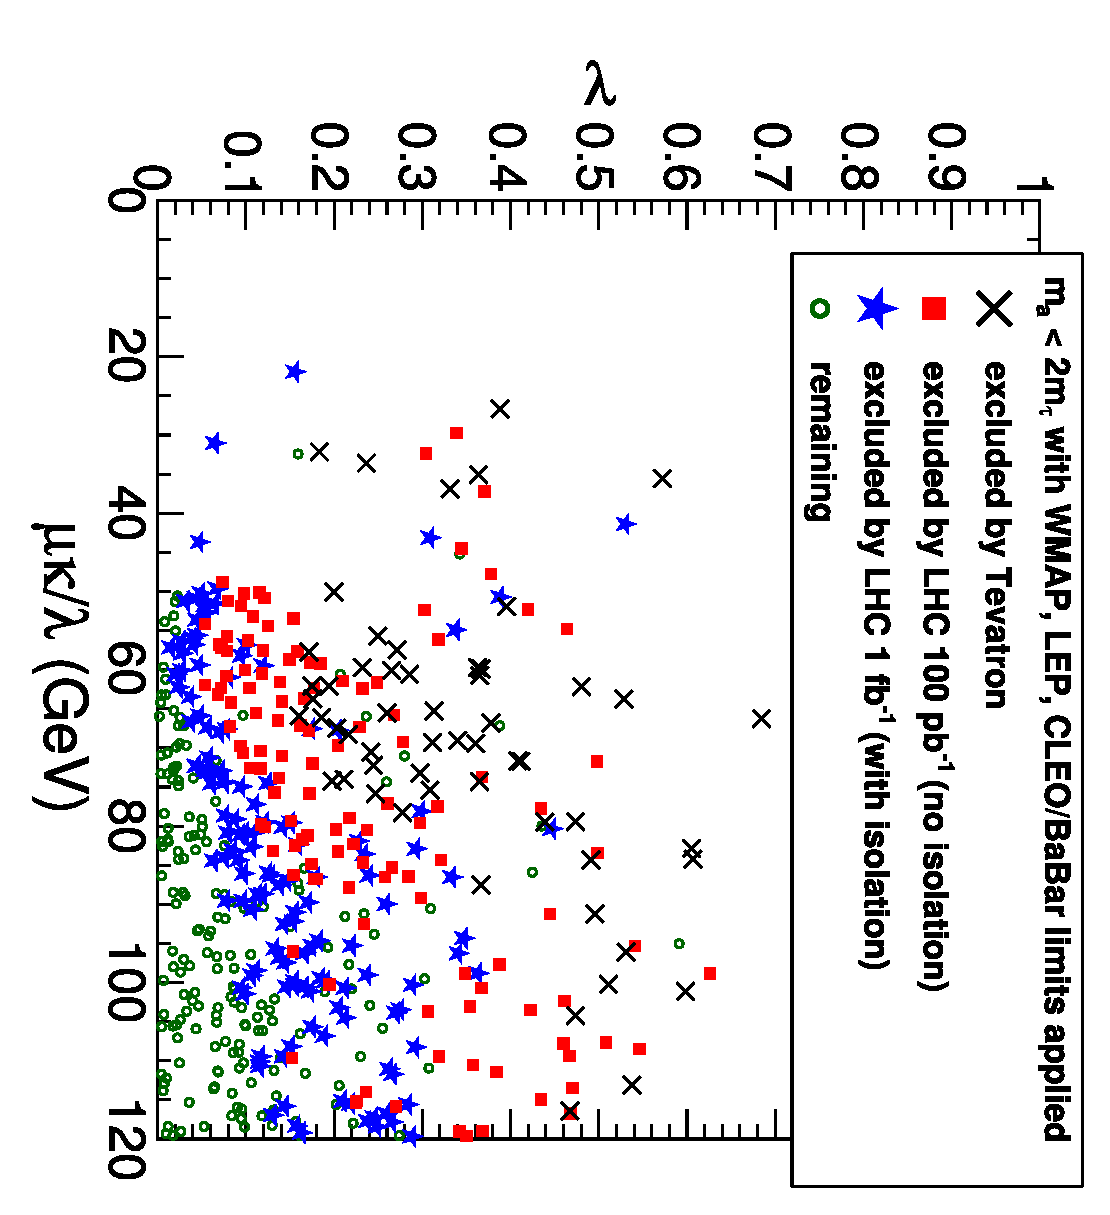
\includegraphics[height=0.32\linewidth, angle=90]{plots/newbranching/newlhcconstraints_params.eps}
%%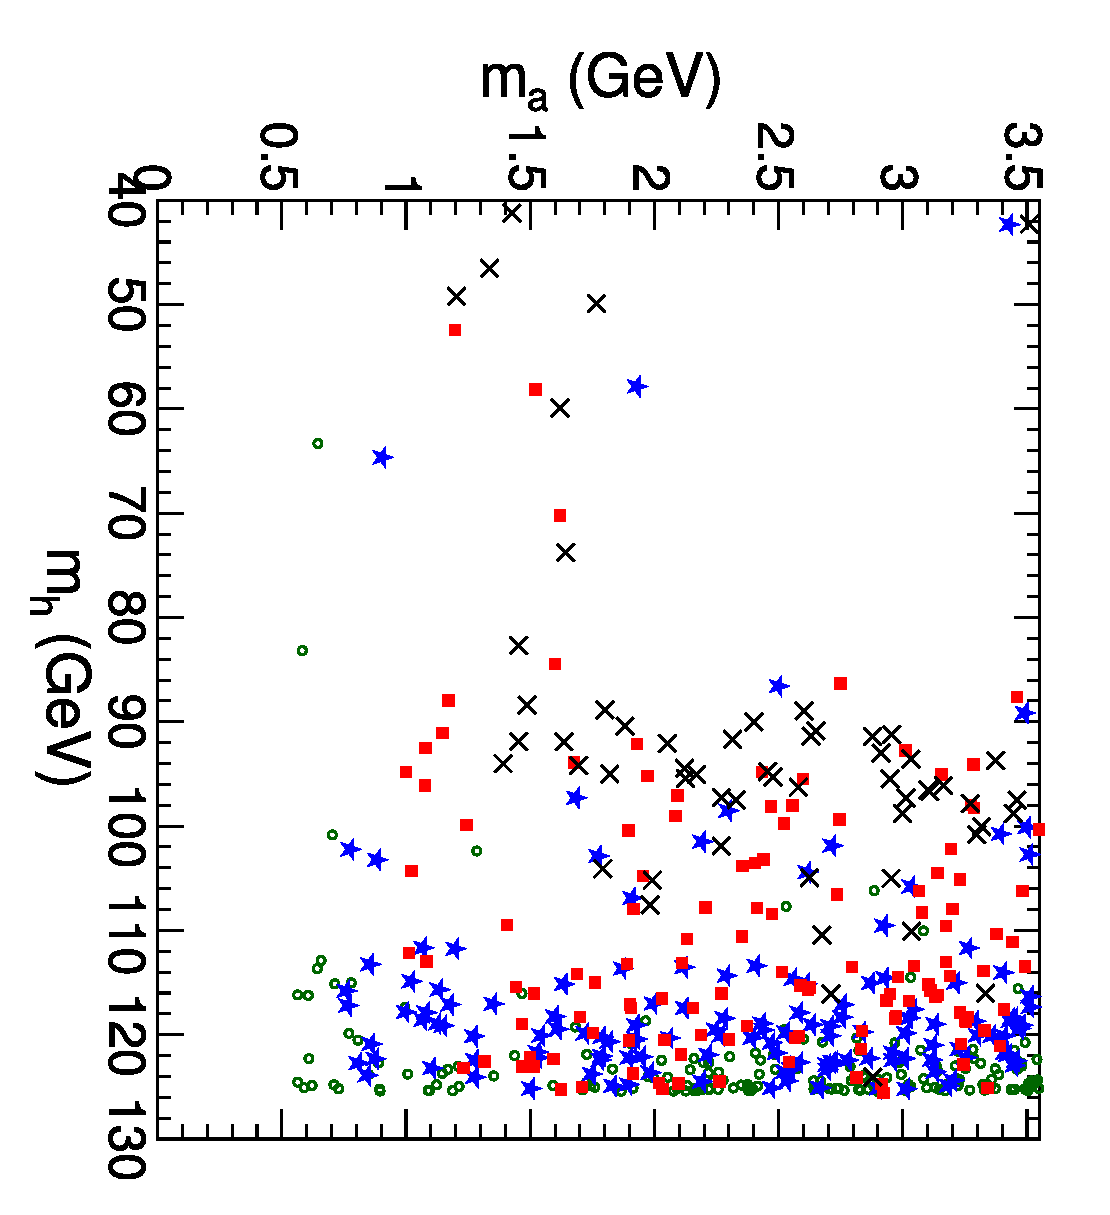
\includegraphics[height=0.32\linewidth, angle=90]{plots/newbranching/newlhcconstraints_masses.eps}
%%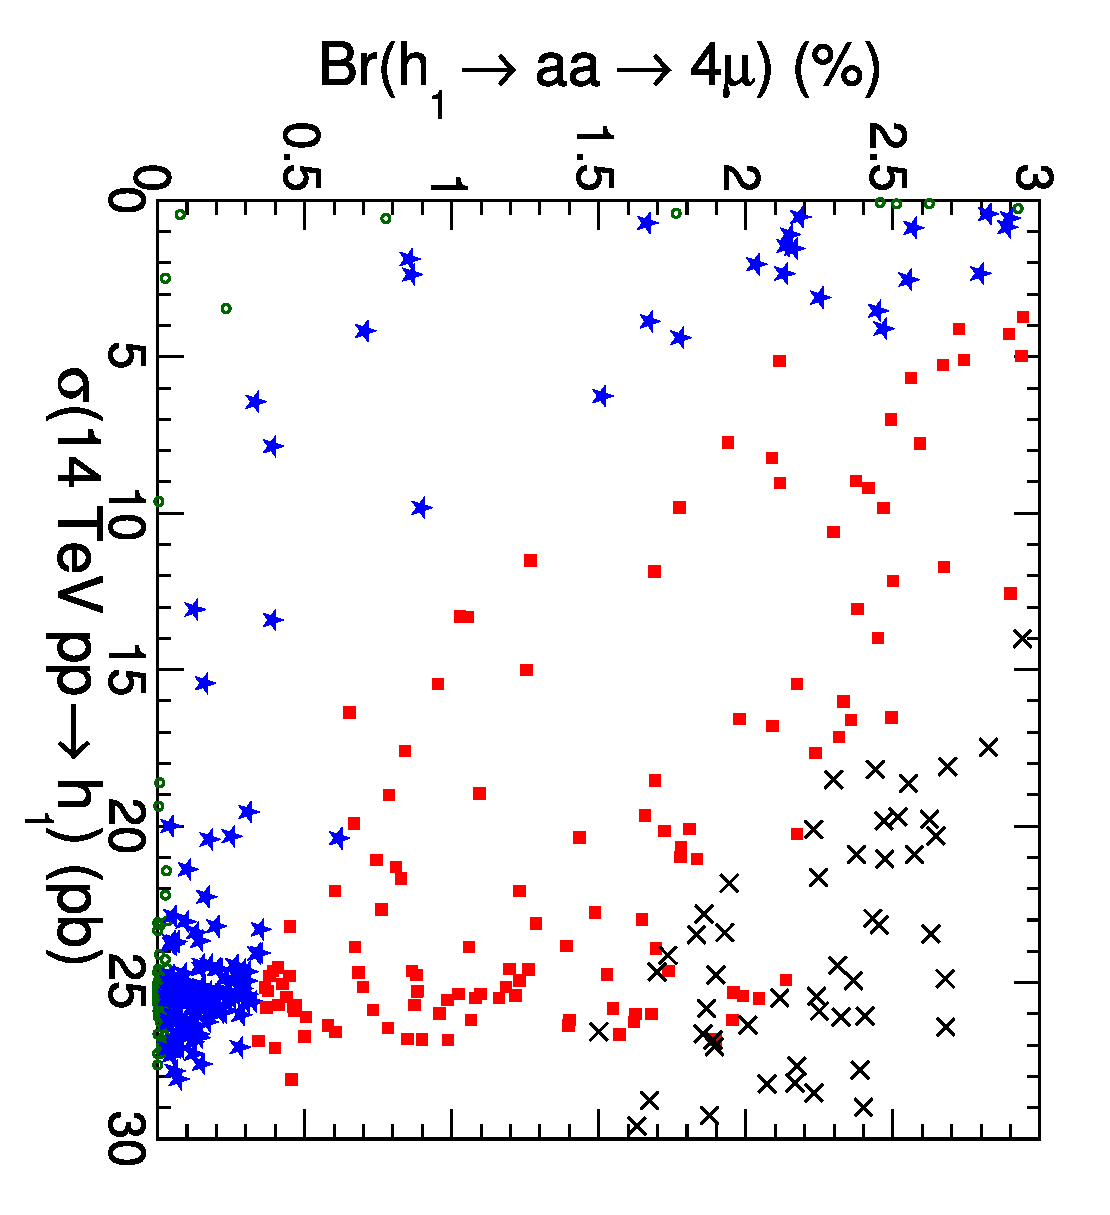
\includegraphics[height=0.32\linewidth, angle=90]{plots/newbranching/newlhcconstraints_crosbr.eps}

\caption{Sampled models excluded by the Tevatron and LHC (with $m_a < 2m_\tau$, WMAP, and LEP constraints applied in all cases).  With only 100~pb$^{-1}$, the LHC's reach extends beyond that of the Tevatron. \label{fig:lhcexclusion}}
\end{figure*}


\section{Results}

{\bf TO BE WRITTEN}

 




%
\section*{Acknowledgments}
We thank 
Ulrich Ellwanger, Cyril Hugonie,
Alexander Pukhov, Jay Wacker
for usefull discussions


%\clearpage
%
%  References
%

%%%%%%%%%%%%%%%%%%%%%%%%%%%% References section %%%%%%%%%%%%%%%%%%%%%%%%%%
% A useful Journal macro
\def\Journal#1#2#3#4{{#1} {\bf #2}, #3 (#4)}
% Some useful journal names
\def\NCA{Nuovo Cimento}
\def\NIM{Nucl. Instrum. Methods}
\def\NIMA{{Nucl. Instrum. Methods} A}
\def\NP{Nucl. Phys.} 
\def\NPB{{Nucl. Phys.} B}
\def\PLB{{Phys. Lett.}  B}
\def\PRL{Phys. Rev. Lett.}
\def\RPP{Rep. Prog. Phys.}
\def\PRD{{Phys. Rev.} D}
\def\PR{Phys. Rep.}
\def\PRP{Prog. Theor. Phys.}
\def\ZPC{{Z. Phys.} C}
\def\MPL{{Mod. Phys. Lett.} A}
\def\EPJC{{Eur. Phys. J.} C}
\def\CPC{Comput. Phys. Commun.}

\renewcommand{\baselinestretch}{1}
%\mytableorig

\begin{thebibliography}{99}

\bibitem{Nilles:1982dy}
  H.~P.~Nilles, M.~Srednicki and D.~Wyler,
  %``Weak Interaction Breakdown Induced By Supergravity,''
  Phys.\ Lett.\  B {\bf 120} (1983) 346.
  %%CITATION = PHLTA,B120,346;%%

%\cite{Frere:1983ag}
\bibitem{Frere:1983ag}
  J.~M.~Frere, D.~R.~T.~Jones and S.~Raby,
  %``Fermion Masses And Induction Of The Weak Scale By Supergravity,''
  Nucl.\ Phys.\  B {\bf 222} (1983) 11.
  %%CITATION = NUPHA,B222,11;%%


%\cite{Ellis:1988er}
\bibitem{Ellis:1988er}
  J.~R.~Ellis, J.~F.~Gunion, H.~E.~Haber, L.~Roszkowski and F.~Zwirner,
  %``Higgs Bosons in a Nonminimal Supersymmetric Model,''
  Phys.\ Rev.\  D {\bf 39} (1989) 844.
  %%CITATION = PHRVA,D39,844;%%

%\cite{Drees:1988fc}
\bibitem{Drees:1988fc}
  M.~Drees,
  %``Supersymmetric Models with Extended Higgs Sector,''
  Int.\ J.\ Mod.\ Phys.\  A {\bf 4} (1989) 3635.
  %%CITATION = IMPAE,A4,3635;%%

%\cite{Ellwanger:1993hn}
\bibitem{Ellwanger:1993hn}
  U.~Ellwanger,
  % ``Radiative corrections to the neutral Higgs spectrum in
  %supersymmetry with a gauge singlet,''
  Phys.\ Lett.\  B {\bf 303} (1993) 271
  [arXiv:hep-ph/9302224].
  %%CITATION = PHLTA,B303,271;%%

%\cite{Ellwanger:1993xa}
\bibitem{Ellwanger:1993xa}
  U.~Ellwanger, M.~Rausch de Traubenberg and C.~A.~Savoy,
  %``Particle spectrum in supersymmetric models with a gauge singlet,''
  Phys.\ Lett.\  B {\bf 315} (1993) 331
  [arXiv:hep-ph/9307322].
  %%CITATION = PHLTA,B315,331;%%

%\cite{Elliott:1993bs}
\bibitem{Elliott:1993bs}
  T.~Elliott, S.~F.~King and P.~L.~White,
  % ``Radiative corrections to Higgs boson masses in the next-to-minimal
  %supersymmetric Standard Model,''
  Phys.\ Rev.\  D {\bf 49} 2435 (1994) 2435
  [arXiv:hep-ph/9308309].
  %%CITATION = PHRVA,D49,2435;%%

%\cite{Pandita:1993tg}
\bibitem{Pandita:1993tg}
  P.~N.~Pandita,
  % ``Radiative corrections to the scalar Higgs masses in a nonminimal
  %supersymmetric Standard Model,''
  Z.\ Phys.\  C {\bf 59} (1993) 575.
  %%CITATION = ZEPYA,C59,575;%%

%\cite{Ellwanger:1995ru}
\bibitem{Ellwanger:1995ru}
  U.~Ellwanger, M.~Rausch de Traubenberg and C.~A.~Savoy,
  %``Higgs phenomenology of the supersymmetric model with a gauge singlet,''
  Z.\ Phys.\  C {\bf 67} (1995) 665
  [arXiv:hep-ph/9502206].
  %%CITATION = ZEPYA,C67,665;%%

%\cite{King:1995vk}
\bibitem{King:1995vk}
  S.~F.~King and P.~L.~White,
  % ``Resolving the constrained minimal and next-to-minimal supersymmetric
  %standard models,''
  Phys.\ Rev.\  D {\bf 52} (1995) 4183
  [arXiv:hep-ph/9505326].
  %%CITATION = PHRVA,D52,4183;%%

%\cite{Franke:1995tc}
\bibitem{Franke:1995tc}
  F.~Franke and H.~Fraas,
  % ``Neutralinos and Higgs Bosons in the Next-To-Minimal
  % Supersymmetric Standard Model,''
  Int.\ J.\ Mod.\ Phys.\  A {\bf 12} (1997) 479
  [arXiv:hep-ph/9512366].
  %%CITATION = IMPAE,A12,479;%%

%\cite{Ellwanger:1996gw}
\bibitem{Ellwanger:1996gw}
  U.~Ellwanger, M.~Rausch de Traubenberg and C.~A.~Savoy,
  %``Phenomenology of supersymmetric models with a singlet,''
  Nucl.\ Phys.\  B {\bf 492} (1997) 21
  [arXiv:hep-ph/9611251].
  %%CITATION = NUPHA,B492,21;%%


\bibitem{Miller:2003ay}
  D.~J.~Miller, R.~Nevzorov and P.~M.~Zerwas,
  %``The Higgs sector of the next-to-minimal supersymmetric standard model,''
  Nucl.\ Phys.\  B {\bf 681} (2004) 3.
%  [arXiv:hep-ph/0304049].
  %%CITATION = NUPHA,B681,3;%%
  
\bibitem{mu-problem}
J.~E.~Kim and H.~P.~Nilles,
  %``The Mu Problem And The Strong CP Problem,''
  Phys.\ Lett.\  B {\bf 138}, 150 (1984).

\bibitem{Dermisek:2005ar}
  R.~Dermisek and J.~F.~Gunion,
  %``Escaping the large fine tuning and little hierarchy problems in the  next
  %to minimal supersymmetric model and h --> a a decays,''
  Phys.\ Rev.\ Lett.\  {\bf 95}, 041801 (2005)
  [arXiv:hep-ph/0502105].

\bibitem{nmssm-ph1}
B.~A.~Dobrescu, G.~L.~Landsberg and K.~T.~Matchev,
  %``Higgs boson decays to CP-odd scalars at the Tevatron and beyond,''
  Phys.\ Rev.\  D {\bf 63}, 075003 (2001)
  [arXiv:hep-ph/0005308];
%
 B.~A.~Dobrescu and K.~T.~Matchev,
  %``Light axion within the next-to-minimal supersymmetric standard model,''
  JHEP {\bf 0009}, 031 (2000)
  [arXiv:hep-ph/0008192].
  
\bibitem{nmssm-ph2}
 J.~F.~Gunion, H.~E.~Haber and T.~Moroi,
  %``Will at least one of the Higgs bosons of the next-to-minimal
  %supersymmetric extension of the standard model be observable at LEP2  or the
  %LHC?,''
{\it In the Proceedings of 1996 DPF / DPB Summer Study on New Directions for High-Energy Physics (Snowmass 96), Snowmass, Colorado, 25 Jun - 12
Jul 1996, pp LTH095}
  [arXiv:hep-ph/9610337];
  %
  U.~Ellwanger, J.~F.~Gunion and C.~Hugonie,
  %``Establishing a no-lose theorem for NMSSM Higgs boson discovery at the
  %LHC,''
  arXiv:hep-ph/0111179
  
\bibitem{nmssm-ph2b}
   %
 J.~R.~Ellis, J.~F.~Gunion, H.~E.~Haber, L.~Roszkowski and F.~Zwirner,
  %``Higgs Bosons in a Nonminimal Supersymmetric Model,''
  Phys.\ Rev.\  D {\bf 39}, 844 (1989);
  %
  B.~A.~Dobrescu, G.~L.~Landsberg and K.~T.~Matchev,
  %``Higgs boson decays to CP-odd scalars at the Tevatron and beyond,''
  Phys.\ Rev.\  D {\bf 63}, 075003 (2001)
  [arXiv:hep-ph/0005308];
  
    U.~Ellwanger, J.~F.~Gunion, C.~Hugonie and S.~Moretti,
  %``Towards a no-lose theorem for NMSSM Higgs discovery at the LHC,''
  arXiv:hep-ph/0305109;
  %
   %
  U.~Ellwanger, J.~F.~Gunion, C.~Hugonie and S.~Moretti,
  %``NMSSM Higgs discovery at the LHC,''
  %
  arXiv:hep-ph/0401228;
    U.~Ellwanger, J.~F.~Gunion and C.~Hugonie,
  %``Difficult scenarios for NMSSM Higgs discovery at the LHC,''
  JHEP {\bf 0507}, 041 (2005)
  [arXiv:hep-ph/0503203].
  
 
  
\bibitem{nmssm-ph3}
  S.~Moretti, S.~Munir and P.~Poulose,
  %``Another step towards a no-lose theorem for NMSSM Higgs discovery at the
  %LHC,''
  Phys.\ Lett.\  B {\bf 644}, 241 (2007)
  [arXiv:hep-ph/0608233];
  
  
  
\bibitem{nmssm-ph4}
 S.~Chang, P.~J.~Fox and N.~Weiner,
  %``Visible cascade Higgs decays to four photons at hadron colliders,''
  Phys.\ Rev.\ Lett.\  {\bf 98}, 111802 (2007)
  [arXiv:hep-ph/0608310]. 
  
\bibitem{nmssm-ph5}
  R.~Dermisek and J.~F.~Gunion,
  %``The NMSSM close to the R-symmetry limit and naturalness in h --> aa  decays
  %for m(a) < 2m(b),''
  Phys.\ Rev.\  D {\bf 75}, 075019 (2007)
  [arXiv:hep-ph/0611142].  
  
\bibitem{nmssm-ph6}
 K.~Cheung, J.~Song and Q.~S.~Yan,
  %``Role of h --> eta eta in Intermediate-Mass Higgs Boson Searches at the
  %Large Hadron Collider,''
  Phys.\ Rev.\ Lett.\  {\bf 99}, 031801 (2007)
  [arXiv:hep-ph/0703149]. 

\bibitem{nmssm-ph6a}  
  J.~R.~Forshaw, J.~F.~Gunion, L.~Hodgkinson, A.~Papaefstathiou and A.~D.~Pilkington,
  %``Reinstating the 'no-lose' theorem for NMSSM Higgs discovery at the LHC,''
  JHEP {\bf 0804} (2008) 090
  [arXiv:0712.3510 [hep-ph]].  
  
\bibitem{nmssm-ph7}
  A.~Belyaev, S.~Hesselbach, S.~Lehti, S.~Moretti, 
  A.~Nikitenko and C.~H.~Shepherd-Themistocleous,
  %``The Scope of the 4 tau Channel in Higgs-strahlung and Vector Boson Fusion
  %for the NMSSM No-Lose Theorem at the LHC,''
  arXiv:0805.3505 [hep-ph]. 
  
\bibitem{nmssm-dm}
A.~Menon, D.~E.~Morrissey and C.~E.~M.~Wagner,
  %``Electroweak baryogenesis and dark matter in the nMSSM,''
  Phys.\ Rev.\  D {\bf 70} (2004) 035005
  [arXiv:hep-ph/0404184];
  D.~G.~Cerdeno, C.~Hugonie, D.~E.~Lopez-Fogliani, C.~Munoz and A.~M.~Teixeira,
  %``Theoretical predictions for the direct detection of neutralino dark  matter
  %in the NMSSM,''
  JHEP {\bf 0412} (2004) 048
  [arXiv:hep-ph/0408102];
  %
  G.~Belanger, F.~Boudjema, C.~Hugonie, A.~Pukhov and A.~Semenov,
  %``Relic density of dark matter in the NMSSM,''
  JCAP {\bf 0509}, 001 (2005)
  [arXiv:hep-ph/0505142];
  %
  J.~F.~Gunion, D.~Hooper and B.~McElrath,
  %``Light neutralino dark matter in the NMSSM,''
  Phys.\ Rev.\  D {\bf 73}, 015011 (2006)
  [arXiv:hep-ph/0509024];
  %
  F.~Ferrer, L.~M.~Krauss and S.~Profumo,
  %``Indirect detection of light neutralino dark matter in the NMSSM,''
  Phys.\ Rev.\  D {\bf 74}, 115007 (2006)
  [arXiv:hep-ph/0609257];
  %
   D.~G.~Cerdeno, E.~Gabrielli, D.~E.~Lopez-Fogliani, C.~Munoz and A.~M.~Teixeira,
  %``Phenomenological viability of neutralino dark matter in the NMSSM,''
  JCAP {\bf 0706}, 008 (2007)
  [arXiv:hep-ph/0701271];
  %
  C.~Hugonie, G.~Belanger and A.~Pukhov,
  %``Dark Matter in the Constrained NMSSM,''
  JCAP {\bf 0711}, 009 (2007)
  [arXiv:0707.0628 [hep-ph]];
  %
  V.~Barger, P.~Langacker, I.~Lewis, M.~McCaskey, G.~Shaughnessy and B.~Yencho,
  %``Recoil detection of the lightest neutralino in MSSM singlet extensions,''
  Phys.\ Rev.\  D {\bf 75}, 115002 (2007)
  [arXiv:hep-ph/0702036].
  %
  S.~Kraml, A.~R.~Raklev and M.~J.~White,
  %``NMSSM in disguise: discovering singlino dark matter with soft leptons at
  %the LHC,''
  Phys.\ Lett.\  B {\bf 672}, 361 (2009)
  [arXiv:0811.0011 [hep-ph]];
  %
  G.~Belanger, C.~Hugonie and A.~Pukhov,
  %``Precision measurements, dark matter direct detection and LHC Higgs searches
  %in a constrained NMSSM,''
  JCAP {\bf 0901}, 023 (2009)
  [arXiv:0811.3224 [hep-ph]].
  


\bibitem{nmssmtools1} U.~Ellwanger, J.F.~Gunion and C.~Hugoine,
\Journal{JHEP}{0502}{066}{2005}.

\bibitem{nmssmtools2} U.~Ellwanger, C.~Hugoine, \Journal{\CPC}{175}{290}{2006}.

\bibitem{nmssmtools3} F.~Domingo and U.~Ellwanger, arXiv:0710.3714 [hep-ph].

\bibitem{wmap}
  D.~N.~Spergel {\it et al.}  [WMAP Collaboration],
  %``First Year Wilkinson Microwave Anisotropy Probe (WMAP) Observations:
  %Determination of Cosmological Parameters,''
  Astrophys.\ J.\ Suppl.\  {\bf 148}, 175 (2003)
  [arXiv:astro-ph/0302209];
%
  C.~L.~Bennett {\it et al.}  [WMAP Collaboration],
  %``First Year Wilkinson Microwave Anisotropy Probe (WMAP) Observations:
  %Preliminary Maps and Basic Results,''
  Astrophys.\ J.\ Suppl.\  {\bf 148}, 1 (2003)
  [arXiv:astro-ph/0302207];
%
  D.~N.~Spergel {\it et al.}  [WMAP Collaboration],
  %``Wilkinson Microwave Anisotropy Probe (WMAP) three year results:
  %Implications for cosmology,''
  Astrophys.\ J.\ Suppl.\  {\bf 170}, 377 (2007)
  [arXiv:astro-ph/0603449].  

%\cite{Abazov:2009yi}
\bibitem{Abazov:2009yi}
  V.~M.~Abazov {\it et al.}  [D0 Collaboration],
  %``Search for NMSSM Higgs bosons in the h->aa->mumu mumu, mumu tautau channels
  %using ppbar collisions at sqrt{s}=1.96 TeV,''
  Phys.\ Rev.\ Lett.\  {\bf 103}, 061801 (2009)
  [arXiv:0905.3381 [hep-ex]].
  %%CITATION = PRLTA,103,061801;%%

\bibitem{lep1exclusion} G.~Abbiendi~\etal (OPAL Collaboration),
\Journal{\EPJC}{18}{425-445}{2001}.

\bibitem{lep2exclusion} G.~Abbiendi~\etal (OPAL Collaboration),
\Journal{\EPJC}{27}{483-495}{2003}, arXiv:0209068v1 [hep-ex].

\bibitem{:2008hs}
  W.~Love {\it et al.}  [CLEO Collaboration],
  %``Search for Very Light CP-Odd Higgs Boson in Radiative Decays of
  %Upsilon(S-1),''
  Phys.\ Rev.\ Lett.\  {\bf 101}, 151802 (2008)
  [arXiv:0807.1427 [hep-ex]].
  %%CITATION = PRLTA,101,151802;%%

\bibitem{Aubert:2009cp}
  B.~Aubert {\it et al.}  [BABAR Collaboration],
  %``Search for Dimuon Decays of a Light Scalar Boson in Radiative Transitions
  %Upsilon -> gamma A0,''
  Phys.\ Rev.\ Lett.\  {\bf 103}, 081803 (2009)
  [arXiv:0905.4539 [hep-ex]].
%\cite{Spira:1995rr}

\bibitem{Ellwanger:2009dp}
  U.~Ellwanger, C.~Hugonie and A.~M.~Teixeira,
  %``The Next-to-Minimal Supersymmetric Standard Model,''
  arXiv:0910.1785 [hep-ph].

\bibitem{Spira:1995rr}
  M.~Spira, A.~Djouadi, D.~Graudenz and P.~M.~Zerwas,
  %``Higgs boson production at the LHC,''
  Nucl.\ Phys.\  B {\bf 453}, 17 (1995)
  [arXiv:hep-ph/9504378].
  %%CITATION = NUPHA,B453,17;%%%\cite{Spira:1995mt}

 %\cite{Djouadi:1997yw}
\bibitem{Djouadi:1997yw}
  A.~Djouadi, J.~Kalinowski and M.~Spira,
  %``HDECAY: A program for Higgs boson decays in the standard model and its
  %supersymmetric extension,''
  Comput.\ Phys.\ Commun.\  {\bf 108}, 56 (1998)
  [arXiv:hep-ph/9704448].
  %%CITATION = CPHCB,108,56;%% 

%\cite{Balazs:1998sb}
\bibitem{Balazs:1998sb}
  C.~Balazs, H.~J.~He and C.~P.~Yuan,
  %``QCD corrections to scalar production via heavy quark fusion at hadron
  %colliders,''
  Phys.\ Rev.\  D {\bf 60}, 114001 (1999)
  [arXiv:hep-ph/9812263].
  %%CITATION = PHRVA,D60,114001;%%
  
  
 %\cite{Belyaev:2005nu}
\bibitem{Belyaev:2005nu}
  A.~Belyaev, J.~Pumplin, W.~K.~Tung and C.~P.~Yuan,
  %``Uncertainties of the inclusive Higgs production cross section at the
  %Tevatron and the LHC,''
  JHEP {\bf 0601}, 069 (2006)
  [arXiv:hep-ph/0508222].
  %%CITATION = JHEPA,0601,069;%% 

%\cite{cleo-low-ma}
\bibitem{cleo-low-ma} (CLEO Collaboration) Phys.\ Rev.\ D {\bf 76}, 117102 (2007); 

%\cite{babar-low-ma}
\bibitem{babar-low-ma} (BaBar) Phys. Rev. Lett. 103:081803 (2009);

%\cite{babar-low-ma}
\bibitem{d0-low-ma} PRL 103, 061801 (2009).

%\cite{micrOmegas}
\bibitem{micrOmegas} G. Belanger, F. Boudjema, C. Hugonie, A. Pukhov, A. Semenov, JCAP 0509:001 (2005), arXiv:hep-ph/0505142

%\cite{LHiggsADecays}
\bibitem{LHiggsADecays} K. Cheung, J. Song, P. Tsong, Q.-S. Yan, Phys.\ Rev.\ D {\bf 78}, 055015 (2008), arXiv:hep-ph/0806.4411; 

%\cite{4mu_pheno}
\bibitem{4mu_pheno} Mariangela Lisanti, Jay G. Wacker, Published in Phys.\ Rev.\ D{\bf 79}:115006, (2009), arXiv:0903.1377;


  
%
% Coordinate for CDF detector
%

%\bibitem{CDFdet} CDF Collaboration, F.~Abe~\etal, \Journal{\NIMA}{271}{387}{1988}.
    
%\bibitem{Topref} CDF Collaboration, F.~Abe~\etal, \Journal{\PRD}{50}{2966}{1994}.
\end{thebibliography}

\end{document}

\bibitem{Djouadi:2008uw}
  A.~Djouadi {\it et al.},
  %``Benchmark scenarios for the NMSSM,''
  arXiv:0801.4321 [hep-ph].
  %%CITATION = ARXIV:0801.4321;%%

%\cite{Djouadi:2008yj}
\bibitem{Djouadi:2008yj}
  A.~Djouadi, U.~Ellwanger and A.~M.~Teixeira,
  %``The constrained next-to-minimal supersymmetric standard model,''
  arXiv:0803.0253 [hep-ph].
  %%CITATION = ARXIV:0803.0253;%%

\bibitem{cNMSSM-benchmarks} 
A. Djouadi, U. Ellwanger, R. Godbole,  
C. Hugonie,  S.F. King,  S. Lehti, 
S. Moretti, A. Nikitenko, 
I. Rottl\"ander,  M. Schumacher and 
A. M. Teixeira, in arXiv:0803.1154 [hep-ph].
